\documentclass[12pt,oneside]{book}

%============================================================
% PACKAGES
%============================================================

%--------------------
% Page + font
%--------------------
\usepackage[margin=1in]{geometry}
\usepackage[T1]{fontenc}
\usepackage[utf8]{inputenc}
\usepackage{lmodern}
\usepackage{microtype}
\usepackage{parskip}


%--------------------
% Math
%--------------------
\usepackage{amsmath, amssymb, amsfonts, amsthm, mathtools}
\usepackage{bm}
\usepackage{bbm}
\usepackage{mathrsfs}
\usepackage{dsfont}

%--------------------
% Tables + figures
%--------------------
\usepackage{graphicx}
\usepackage{float}
\usepackage{booktabs}
\usepackage{array}
\usepackage{xltabular}
\usepackage{multirow}
\usepackage{caption}
\usepackage{subcaption}
\usepackage{tikz}

%--------------------
% Lists
%--------------------
\usepackage{enumitem}
\setlist[itemize]{topsep=2pt,itemsep=2pt}
\setlist[enumerate]{topsep=2pt,itemsep=2pt}

%--------------------
% Colors + hyperlinks
%--------------------
\usepackage[dvipsnames]{xcolor}
\usepackage[
    colorlinks=true,
    linkcolor=MidnightBlue,
    citecolor=MidnightBlue,
    urlcolor=MidnightBlue
]{hyperref}
\usepackage[nameinlink,capitalise]{cleveref}

%--------------------
% Algorithms
%--------------------
\usepackage{algorithm}
\usepackage{algpseudocode}

%--------------------
% Code blocks
%--------------------
\usepackage{listings}

\lstdefinestyle{codestyle}{
    basicstyle=\ttfamily\small,
    breaklines=true,
    frame=single,
    numbers=left,
    numberstyle=\tiny,
    keywordstyle=\color{MidnightBlue},
    commentstyle=\color{ForestGreen},
    stringstyle=\color{BrickRed},
    showstringspaces=false,
    tabsize=4
}

\lstset{style=codestyle}

%--------------------
% Section styling
%--------------------
\usepackage{titlesec}
\usepackage{tocloft}

\setcounter{tocdepth}{2}
\setcounter{secnumdepth}{3}

%============================================================
% THEOREMS
%============================================================

\numberwithin{equation}{section}

\theoremstyle{definition}
\newtheorem{definition}{Definition}[section]
\newtheorem{example}{Example}[section]
\newtheorem{exercise}{Exercise}[section]
\newtheorem{remark}{Remark}[section]

\theoremstyle{plain}
\newtheorem{theorem}{Theorem}[section]
\newtheorem{lemma}{Lemma}[section]
\newtheorem{proposition}{Proposition}[section]
\newtheorem{corollary}{Corollary}[section]

\theoremstyle{remark}
\newtheorem*{note}{Note}

%============================================================
% CUSTOM COMMANDS
%============================================================

% Sets
\newcommand{\R}{\mathbb{R}}
\newcommand{\N}{\mathbb{N}}
\newcommand{\Z}{\mathbb{Z}}
\newcommand{\Q}{\mathbb{Q}}
\newcommand{\C}{\mathbb{C}}
\newcommand{\powerset}{\mathcal{P}}


% Probability
\newcommand{\E}{\mathbb{E}}
\newcommand{\Var}{\mathrm{Var}}
\newcommand{\Cov}{\mathrm{Cov}}
\newcommand{\Corr}{\mathrm{Corr}}
\newcommand{\Prob}{\mathbb{Pr}}

\newcommand{\ind}{\mathbbm{1}}
\newcommand{\iid}{\overset{\text{iid}}{\sim}}
\newcommand{\convd}{\overset{d}{\to}}
\newcommand{\convp}{\overset{p}{\to}}
\newcommand{\as}{\overset{a.s.}{\to}}

% Operators
\newcommand{\given}{\,\middle|\,}
\newcommand{\argmin}{\operatorname*{arg\,min}}
\newcommand{\argmax}{\operatorname*{arg\,max}}

% Linear algebra / analysis
\newcommand{\norm}[1]{\left\lVert #1 \right\rVert}
\newcommand{\abs}[1]{\left\lvert #1 \right\rvert}
\newcommand{\inner}[2]{\left\langle #1, #2 \right\rangle}

\newcommand{\dd}{\,\mathrm{d}}
\newcommand{\grad}{\nabla}
\newcommand{\Hess}{\nabla^2}

\newcommand{\tr}{\operatorname{tr}}
\newcommand{\rank}{\operatorname{rank}}
\newcommand{\diag}{\operatorname{diag}}

% Distributions
\newcommand{\Normal}{\mathcal{N}}
\newcommand{\Bern}{\mathrm{Bernoulli}}
\newcommand{\Bin}{\mathrm{Binomial}}
\newcommand{\Pois}{\mathrm{Poisson}}
\newcommand{\Gam}{\mathrm{Gamma}}
\newcommand{\BetaDist}{\mathrm{Beta}}
\newcommand{\Exp}{\mathrm{Exponential}}
\newcommand{\Dir}{\mathrm{Dirichlet}}
\newcommand{\InvGam}{\mathrm{Inv\text{-}Gamma}}

%============================================================
% TITLE INFO
%============================================================

\title{EN.553.740 Machine Learning 1}
\author{Jonathan Ma}
\date{\today}

%============================================================
% DOCUMENT
%============================================================

\begin{document}

\maketitle
\tableofcontents

\section{Introduction}
A good way to think of machine learning is instead of a computer taking data and a program to produce output, it takes data and output and attempts to produce a program, ie "learn" a function.

We use it for tasks that are too complex to program, like driving or large scale data analysis. A bit of history of "learning":
\begin{itemize}
    \item 1959: Arthur Samuel (IBM) created a program to play checkers, introducing rule-based learning.
    \item 1960: Frank Rosenblatt introduced a linear classifier based on brain neurons, called a Perceptron.
    \item 1969: Marvin Minsky showed limitations of the perceptron, halting development for 20 years
    \item 1980: First workshop in machine learning
    \item 1986: Multilayer networks and backpropagation introduced
    \item 1990: Vapnik and Chervonenkis introduce kernels and SVM, and termed "Statistical Learning"
    \item 2002: Rise of graphical models
    \item 2010: Deep learning takes over
    \item 2016: ML hits record size with NIPS and ICML doubling in size
\end{itemize}

Machine learning has been used for a variety of tasks, like stock market prediction, decoding thoughts from brain scans, and self-driving cars.

\subsection{Learning Problems}
Statistical Learning falls under five rough fields:
\begin{itemize}
    \item Classification (Assign a category)
    \item Regression (predict a real value)
    \item Ranking (order items)
    \item Clustering (item partitioning, like image segmentation)
    \item Dimensionality Reduction/Manifold Learning (Computer vision)
\end{itemize}
In a broader sense, there is supervised learning (Classification/regression) and unsupervised learning (Clustering, dimensionality reduction, density estimation) and things like semi-supervised learning, active learning, reinforcement learning, etc.

\paragraph{Supervised Learning}
For a given problem, we learn a function $f: X \rightarrow Y$ such that $x \in \mathcal{X}, \quad y \in \mathcal{Y}$. Classification deals with discrete labels while regression deals with continuous functions.

\paragraph{Unsupervised Learning}
For a given problem, we learn a function $f: X \rightarrow Y$ such that $x \in \mathcal{X}, \quad f(x) \in \R$. Usually embedding (for text), clustering, or density estimation.

\section{Mathematical Review}
Algorithms are built from sets, functions, vectors, matrices, norms, and derivatives, so we introduce common notation here. Consider a student success dataset with the target being quiz score, and features as study time and prior score.

\subsection{Linear Algebra}

\subsubsection{Sets and Power Sets}
Let $A = \{1,2,3,4,5\}$ be the set of students in the toy dataset. The \emph{power set} is $\powerset(A)=\{B: B \subseteq A\}$. If $|A|<\infty$, then $|\powerset(A)|=2^{|A|}$. A subset $B \subseteq A$ may represent a mini-batch, validation set, or a selected group of samples.

\subsubsection{Functions}
For sets $A,B$, write $B^A=\{f: A\rightarrow B\}$. if $B=\R$, then $\R^A$ is the set of real-valued functions on $A$. If $|A| < \infty$, then $\R^A \simeq \R^{|A|}$ as vector spaces. For our toy example: \[x_1: A \rightarrow \R \qquad x_2: A \rightarrow \R \qquad y: A \rightarrow \R\]
For a subset $C \subseteq A$, define an \emph{indicator function}:
\[
\mathbbm{1}_C: A \rightarrow \{0,1\}, \quad \mathbbm{1}_C(i)=
\begin{cases}
    1, i \in C, \\
    0, i \notin C
\end{cases}
\]
Indicators are used to encode events, groups, labels, masks, etc.

\subsubsection{Vectors}
We use a column convention for vectors. For each student $i$, write the feature vector as:
\[
x_i = 
\begin{bmatrix}
    x_i^{(1)} \\
    x_i^{(2)} 
\end{bmatrix}
\in \R^2
\]
Standard vectors that are useful include the zero vector ($0_d$), unit vector ($\mathbbm{1}_d$), and identity matrix ($I_{\R^d}$):
\[
0_d=
\begin{bmatrix}
    0 \\
    \vdots \\
    0
\end{bmatrix}
\quad
\mathbbm{1}_d=
\begin{bmatrix}
    1 \\
    \vdots \\
    1
\end{bmatrix}
\quad
I_{\R^d}=
\begin{bmatrix}
    1 \cdots 0 \\
    \quad \ddots \quad \\
    0 \cdots 1
\end{bmatrix}
\]
\subsubsection{$\ell^p$ norms}
For $p \ge 1$ and $x \in \R^d$, a $p$-norm is defined as \[\norm{x}_p = (|x^{(1)}|^p + \cdots + |x^{(d)}|^p)^{\frac{1}{p}}\]. Special cases include:
\[\ell_1 = \sum_j |x^{(j)}| \quad \ell_2 = \sqrt{\sum_j (x^{(j)})^2} \quad \ell_\infty = \max_j |x^{(j)}|\]
$\ell^2$ is called the euclidean norm. We require $p\ge 1$ because the triangle inequality holding is essential for a norm, and only holds for $p\ge 1$:
\[
\norm{x+y}_p \le \norm{x}_p + \norm{y}_p 
\]
\[
\text{ when } p=1; |x| + |y| \le 1 
\]
\[
\text{ when } p=\infty; \max \{|x|,|y|\} \le 1 \iff |x| \le 1, 
\]
A good visualization of norms is shown below:
% TODO: add a tikz diagram comparing L1, L2, and L infinity norms
\begin{figure}[H]
    \centering
    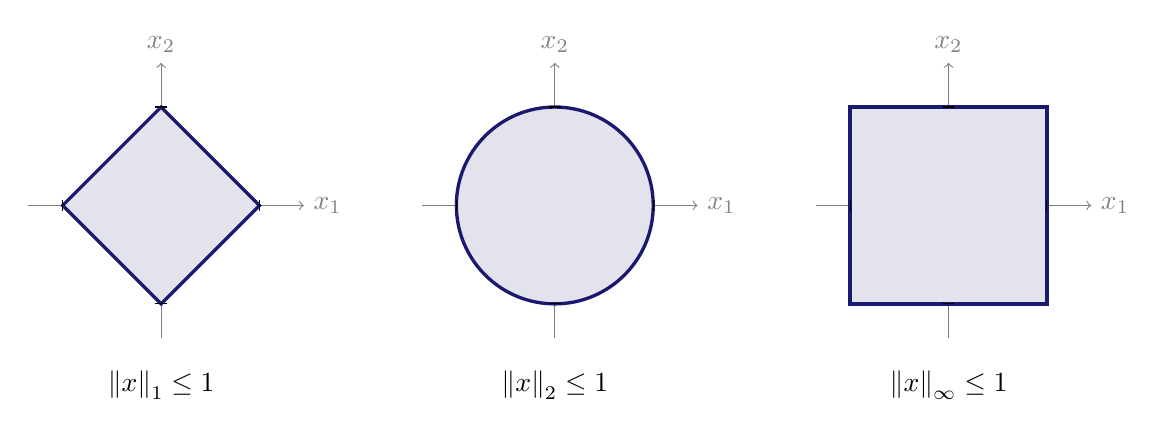
\begin{tikzpicture}[scale=1.25]
        \tikzset{
            axes/.style={->,thin,gray},
            ball/.style={draw=MidnightBlue,very thick,fill=MidnightBlue!12}
        }

        % l_1 unit ball
        \begin{scope}[xshift=0cm]
            \draw[axes] (-1.35,0) -- (1.45,0) node[right] {$x_1$};
            \draw[axes] (0,-1.35) -- (0,1.45) node[above] {$x_2$};
            \draw[ball] (1,0) -- (0,1) -- (-1,0) -- (0,-1) -- cycle;
            \foreach \x in {-1,1} {
                \draw (\x,0.06) -- (\x,-0.06);
                \draw (0.06,\x) -- (-0.06,\x);
            }
            \node[below=8pt] at (0,-1.35)
                {$\norm{x}_1\leq 1$};
        \end{scope}

        % l_2 unit ball
        \begin{scope}[xshift=4cm]
            \draw[axes] (-1.35,0) -- (1.45,0) node[right] {$x_1$};
            \draw[axes] (0,-1.35) -- (0,1.45) node[above] {$x_2$};
            \draw[ball] (0,0) circle (1);
            \foreach \x in {-1,1} {
                \draw (\x,0.06) -- (\x,-0.06);
                \draw (0.06,\x) -- (-0.06,\x);
            }
            \node[below=8pt] at (0,-1.35)
                {$\norm{x}_2\leq 1$};
        \end{scope}

        % l_infinity unit ball
        \begin{scope}[xshift=8cm]
            \draw[axes] (-1.35,0) -- (1.45,0) node[right] {$x_1$};
            \draw[axes] (0,-1.35) -- (0,1.45) node[above] {$x_2$};
            \draw[ball] (-1,-1) rectangle (1,1);
            \foreach \x in {-1,1} {
                \draw (\x,0.06) -- (\x,-0.06);
                \draw (0.06,\x) -- (-0.06,\x);
            }
            \node[below=8pt] at (0,-1.35)
                {$\norm{x}_\infty\leq 1$};
        \end{scope}
    \end{tikzpicture}
    \caption{Unit balls in $\R^2$. Their boundaries consist of vectors with
    norm equal to one.}
    \label{fig:lp-unit-balls}
\end{figure}

\paragraph{Operator Norms}
For $A \in \mathcal{M}_{m,d}$, $\norm{A}_{op} := \max \{\norm{Ax}_2 : x \in \R^d, \norm{x}_2 = 1\}$. $\norm{A}_{op}$ is the largest stretching factor of the linear map $x \mapsto Ax$. Alternatively, we can derive a similar definition:
\[\norm{Ax}_2^2 = \inner{Ax}{Ax}\]
\[\inner{Ax}{Ax} = (Ax)^TAx = x^TA^TAx\]
\[\norm{Ax}_{op}^2 = \max_{\norm{x}_2 = 1} x^TA^TAx\]
Operator norms quantify how much perurbations can be amplified. 

\subsubsection{Cauchy-Schwarz Inequality}
For $x,y \in \R^d$, $|\inner{x}{y}| \le \norm{x}_p\norm{y}_q$ with equality iff $x = \alpha y$ for some scalar $\alpha$ and $\frac{1}{p}+\frac{1}{q}=1$.

\paragraph{Proof sketch:} For any $\alpha \in \R$, 
\[
0 \le \norm{x - \alpha y}_2^2 = \norm{x}_2^2 - 2\alpha \inner{x}{y} + \alpha^2 \norm{y}_2^2
\]
Choosing the best $\alpha$ gives the inequality:
\[\forall \alpha \in \R, \quad \norm{x - \alpha y}_2^2 \ge 0\]
\[\iff \inner{x-\alpha y}{x- \alpha y} \ge 0\]
\[\iff \inner{x}{x} - 2\alpha \inner{x}{y} + \alpha^2 \inner{y}{y} \ge 0\]
\[\iff \norm{x}_2^2 - 2\alpha \inner{x}{y} + \alpha^2 \norm{y}_2^2 \ge 0\]
Without loss of generality, assume $\norm{y}_2 \ge 0$ and take $\alpha = \frac{\norm{x}_2}{\norm{y}_2}$:
\[\implies \norm{x}_2^2 - \frac{2 \inner{x}{y}\norm{x}_2}{\norm{y}_2} + \norm{x}_2 \ge 0\]
\[\norm{x}_2 \norm{y}_2 \ge \inner{x}{y}\]
Equality means $x - \alpha^* y = 0$ so $x = \alpha^* y$.

Cauchy-Schwarz is used in ML to control linear scores, since most models are about estimating weights. A linear model estimates $f_w(x) = \inner{w}{x}$. Cauchy-Schwarz gives 
\[|f_w(x)|=|\inner{w}{x}| \le \norm{w}_2 \norm{x}_2\]
This is saying if features have a bounded norm, and weights have a bounded norm, scores cannot explode. This is why norm constraints and regularization appear throughout learning problems. 
\begin{quote}
    The inner product cannot be larger than length times length
\end{quote}
We now look at a particle sensor example. Suppose independent sensors $X_1, X_2, \cdots , X_n$ estimate the same mean $\mu$:
\[\E (X_i) = \mu \qquad \Var (X_i) = \sigma_i^2 \]
Among weighted averages \[\hat{\mu}=\sum_{i=1}^n w_i X_i\] which weights should we use, keeping $\hat{\mu}$ unbiased? Compute:
\[\E (\hat{\mu})=\E [\sum_i w_i X_i] = \sum_i w_i \E X_i = \sum_i w_i \mu = \mu\]
Thus
\[\E (\hat{\mu}) = \mu \iff \sum_i w_i = 1\]
Because $X_i$ are independent,
\[\Var(\hat{\mu})=\Var(\sum_i w_iX_i)=\sum_i w_i^2 \Var(X_i)=\sum_i w_i^2\sigma_i^2\]
The optimization problem we obtain is therefor minimize $\Var(\hat{\mu}) \text{ s.t. } \sum_i w_i = 1$
since the sum of weights is one, \[1 = (\sum_i w_i)^2 = (\sum_i (w_i \sigma_i)\frac{1}{\sigma_i})^2\]
Now by Cauchy-Schwarz, \[1 = (\sum_i w_i)^2 \le (\sum_i w_i^2 \sigma_i^2) (\sum_i \frac{1}{\sigma_i^2})\]
Recall $|\inner{x}{y}| \le \norm{x}_2 \norm{y}_2$. Therefore \[\Var(\hat{\mu})=\sum_i w_i^2 \sigma_i^2 \ge (\sum_i \sigma_i^{-2})^{-1}\]
This makes it so the elements of $X$ and $y$ are $w_i \sigma_i$ and $1/\sigma_i$ respectively. 

Equality in Cauchy-Schwarz holds when \[w_i \sigma_i \propto \sigma_i^{-1} \implies w_i \propto \frac{1}{\sigma_i^2}\] so we should normalize weights so they sum to one: \[\frac{\frac{1}{\sigma_i^2}}{\sum_{j=1}^n \frac{1}{\sigma_i^2}}\] meaning lower variance sensor implies larger weight. 

\subsubsection{Sparsity and Lasso}
Sparsity is roughly defined as what happens when $p \rightarrow 0$. For a nonzero scalar $a$: 
\[\lim_{p \rightarrow 0} \sum_j \abs{x^{(j)}}^p = \sum_j \lim_{p \rightarrow 0}  \abs{x^{(j)}}^p \therefore \lim_{p\rightarrow 0} \abs{a}^p=1 (\text{ imagine } 
\begin{cases}
    0, x^{(j)}=0 \\
    1, x^{(j)}\ne 0
\end{cases}
)\]
For $a=0, \abs{0}^p=0$. Therefore informally, \[\lim_{p\rightarrow 0} \sum_j \abs{x^{(j)}}^p=\{j : x^{(j)} \ne 0\}=\norm{x}_0\]
The quantity $\norm{x}_0$ counts the number of nonzero entries, but it is not a norm and optimization with it is often difficult. Common times in ML, we replace $\norm{x}_0$ with $\norm{x}_1$ to encourage sparsity while keeping convexity

\subsubsection{Matrices}
In ML, rows often represent samples and columns represent features. we say $\mathcal{M}_{m,d}=\mathcal{M}_{m,d}(\R)=\{m \times d \text{ real matrices }\}$. Additionally $\mathcal{M}_d=\mathcal{M}_{d,d}$. Notation may differ, so remember its always (across, down) ie (i,j)/(r,c)/(m,d)

By this definition, a linear prediction vector is $X_w = [\inner{x_1}{w}, \inner{x_2}{w}, \cdots, \inner{x_i}{w}]^T$.

\paragraph{Symmetric and Positive Semidefinite Matrices}
A symmetric matrix is defined as \[S_d=\{A \in \mathcal{M}_d : A = A^T\}\]
A positive semidefinite matrix (PSD) is defined as \[S_d^+ =\{A \in S_d : x^TAx \ge 0 \quad \forall \quad x \in \R^d\}\] These usually appear as covariance and correlation matrices, and Hessians of convex quadratic objective functions.
A positive definite matrix is defined as \[S_d^{++} =\{A \in S_d : x^TAx > 0 \quad \forall \quad x \ne 0\}\] This usually comes up when doing ridge regressions and finding hessians with a parameter greater than 0. 

\paragraph{Bilinear Forms} A bilinear form is a map $a: \R^d \times \R^d \rightarrow \R$ that is linear in each variable. If $a$ is symmetric (ie $a(x,y)=a(y,x)$) then $a(x,y)=x^TAy$ for some symmetric matrix $A \in S_d$.

Inner products are PSD:
\[a(x,y)=\inner{x}{y}=x^Ty\]
\[a(x,y)=\inner{x}{y}=x^TI_dy\]
\[a(x,x)=x^Tx=\norm{x}_2^2 \ge 0\]

\paragraph{Orthogonal Matrices}
An Orthogonal transformation matrix $O$ is defined as \[O_{m,d}=\{A \in \mathcal{M}_{m,d} : AA^T = I_m\}\] and for $Q \in O_d, Q^TQ=QQ^T=I_d$. The key idea is orthogonal transformations rpeserve euclidean geometry:
\[\norm{Qx}_2^2 = (Qx)^T(Qx)=x^TQ^TQx=x^Tx=\norm{x}_2^2\]
Similarly \[\inner{Qx}{Qy}=x^TQ^TQy=
inner{x}{y}\] Rotations preserve distances and dot products, which matter for PCA, kernels, and preprocessing

\subsubsection{Open and Closed Balls}
We introduce some basic topology. For $x \in \R^d, r > 0$:
A ball is open if \[B(x,r)=\{y \in \R^d: \norm{y-x}_2 < r\}\]
A ball includes the boundary if \[\bar{B}(x,r)=\{y \in \R^d: \norm{y-x}_2 \le r\}\]

A set $U \subset \R^d$ is open if \[\forall x \in U, \qquad \exists r > 0, \qquad B(x,r) \subset U\] A set is closed if its complement is open. The intuition is that inside an open set, every point has a small safety ball around it.

For $A \subset \R^d$, the interior ($\int(A)$) is the largest open set containing $A$, and the closure $cl(a)$ is the smallest closed set containing $A$. We can also think of this as the closure iincluding the boundary whereas the interior doesn't.

\paragraph{Compactness}: A set $K \subset \R^d$ is compact if every sequence of points in $K$ contains a subsequence that converges to a point in $K$. Take for instance (0,1) vs [0,1]:
The requence $x_n = n^{-1}$ lies in (0,1) and converges to 0, but $0 \notin (0,1)$, so (0,1) is not compact. For [0,1], limits of convergent subsequences stay inside the set.

\paragraph{Heine-Borel Theorem} A finite-dimensional Euclidean space: \[K \subset \R^d \text{ compact } \iff K \text{ is closed and bounded.}\] Bounded means $ \exists R > 0 \text{ s.t. } K \subset B(0,R)$. This is special to finite dimensional euclidean spaces, not other spaces.

\paragraph{Weierstrass Extreme Value Theorem} If $K \subset \R^d$ is compact and $f:K \rightarrow \R$ is continuous, then $f$ attains its minimum and maximum on K. Put otherways, \[\exists x_{min}, x_{max} \in K \text{ s.t. } f(x_{min})=\min_{x \in K} f(x), \qquad f(x_{max})=\max_{x \in K} f(x)\] In optimization, we often write $\inf_{w \in K} \ell (w)$. Weierstrass tells us when this minimum is actually achieved. Basically saying that on compact parameter sets, continuous objectives have optimizers. We look at an example:

Look at constrained regression. Consider minimizing least squares over a compact ball \[K_R = \{w \in \R^d : \norm{w}_2 \le R\}\]
The objective is \[\ell (w)=\frac{1}{2n} \norm{Xw-y}_2^2\]
We can prove this by showing $\ell (w)$ is continuous in $w$. Then show that $K_R$ is closed and bounded in $\R^d$. By Heine-Borel, $K_R$ is compact, so by Weierstrass, $\exists \hat{w} \in K_R \text{ s.t. } \ell (\hat{w}) = \min_{w \in K_R} \ell (w)$.

\subsubsection{Metric Spaces} A metric space is a set $\mathcal{B}$ equipped with a distance $ \rho: \mathcal{B} \times \mathcal{B} \rightarrow [0.\infty)$ satisfying $\forall x,y,z \in \mathcal{B}$: 
\[\rho(x,y) \iff x=y\]
\[\rho(x,y) =\rho(y,x)\]
\[\rho(x,z) \le \rho(x,y) + \rho(y,z)\]

For $\mathcal{B} \in \R$ and $\rho: \R \times \R$: $\rho(x,y)=\abs{x-y}$.

For $\mathcal{B} \in \R^d$ and $\rho: \R^d \times \R^d$: $\rho(x,y)=\norm{x-y}_2$.

Metrics formalize dissimilarity between data points. This could be distances between two feature vectors, probability distributions, or functions/signals. Open, Closed, and compactness still make sense in metric spaces, but Heine-Borel may fail. In $\R$, closed and bounded iff compact, but in a general metric space, it does not imply compactness

\subsection{Calculus}

\paragraph{Calculus Notation Map}

\begin{center}
\renewcommand{\arraystretch}{1.2}
\begin{tabular}{@{}>{$}l<{$} p{0.67\textwidth}@{}}
\toprule
\multicolumn{1}{@{}l}{\textbf{Notation}} & \textbf{Meaning in these notes} \\
\midrule
x,y \in \R & one-dimensional points, often with $x<y$ \\
x \in \R^d & deterministic vector or input point \\
e_1,\ldots,e_d & canonical basis of $\R^d$: $e_1=(1,0,...), e_2=(0,1,...)$\\
\partial f & derivative in one dimension \\
\partial_j f & partial derivative along $e_j$ \\
df(x) & differential or Jacobian matrix at $x$ \\
\nabla \mathbin{\cdot} f & divergence, when $f\colon\R^d\to\R^d$ \\
\nabla^2 f & Hessian, for scalar-valued $f$ \\
\Delta f & Laplacian, $\tr(\nabla^2 f)$ \\
\bottomrule
\end{tabular}
\end{center}

\paragraph{Probability Notation Map}

\begin{center}
\renewcommand{\arraystretch}{1.2}
\begin{tabular}{@{}>{$}l<{$} p{0.67\textwidth}@{}}
\toprule
\multicolumn{1}{@{}l}{\textbf{Notation}} & \textbf{Meaning in these notes} \\
\midrule
\Omega & sample space \\
A \subseteq \Omega & event \\
\mathbb{P} & probability function or probability measure \\
(\Omega,\mathbb{P}) & probability space \\
X,Y & random variables (capital letters) \\
x,y & realizations or values of random variables \\
R_X,R_Y & possible values of $X$ and $Y$ \\
{[X=x]} & event $\{\omega\in\Omega:X(\omega)=x\}$ \\
\E[X] & expectation of $X$ \\
\E[Y\mid X=x] & conditional expectation of $Y$ given $X=x$ \\
\bottomrule
\end{tabular}
\end{center}
A model is often a function $f(x)$ and a loss is often a function $\ell (w)$ of parameters $w$. Optimization therefore asks how does $\ell (w)$ change after $w$ is perturbed, or, if we move from $w$ to $w+h$, can we predict whether loss goes down?

\paragraph{Intervals} Assume $x,y \in \R; x > y$. The line segment from $x$ to $y$ is written by $(1-t)x + ty$. Define the intervals as follows:
\[[x,y] := \{(1-t)x+ty: 0 \le t \le 1\}\]
\[[x,y) := \{(1-t)x+ty: 0 \le t < 1\}\]
\[(x,y] := \{(1-t)x+ty: 0 < t \le 1\}\]
\[(x,y) := \{(1-t)x+ty: 0 < t < 1\}\]
The same line segment formula will appear in convexity, Jensen's Inequality, and taylor expansion along a direction.

\subsubsection{1D Derivatives}
Let $f: I \subset \R \rightarrow \R, \quad t \mapsto f(t) \in \R$. The derivative of $f$ at $t_0 \in I$ is \[\partial f (t_0) = \partial f |_{t=t_0} := \lim_{h \rightarrow 0} \frac{f(t_0+h)-f(t_0)}{h} \] when this limit exists. For higher-order derivatives: \[\partial^kf := \partial(\cdots \partial(\partial f)), \quad k\ge 0, \quad k \in \Z^+\] with the convention $\partial^0f := f$. The derivative is the local slope of the function at $t_0$. 

\subsubsection{Higher-Dimensional Derivatives}
Now move to $d > 1$, and let $f: U \subset \R^d \rightarrow \R^m$ and $U$ is \emph{open} (meaning we can move a little around $x$ without immediately leaving the domain).

\subsubsection{Partial Derivates}
Let $e_{1,...,}e_d$ be the canonical basis of $\R^d$. For $1 \le j \le d$: \[\partial_jf(x) := \partial_t(f(x+te_j))|_{t=0}=\lim_{t\rightarrow 0}\frac{f(x+te_j)-f(x)}{t}\]

This means that $e_j$ changes only coordinate $j$ and $x+te_j$ means move from $x$ only along coordinate $j$. The partial derivative measures local change in that coordinate direction. 

For example, let $f(\theta)=f(x,y)=x^2+3xy$. Then $\partial_x f(\theta)=2x+3y$ and $\partial_y f(x)=3y$, and at $\theta = (1,2)^T$, $\partial_x f(\theta)=8$ and $\partial_y f(x)=3$

\subsubsection{Directional Derivatives}
Partial derivatives measure change along the coordinate directions. More generally, for a direction $h\in\R^d$, the \emph{directional derivative} of $f$ at $x$ in the direction $h$ is
\[
\left.\partial_t f(x+th)\right|_{t=0}.
\]
A partial derivative is the special case $h=e_j$, whereas a directional derivative allows any $h\in\R^d$.

In machine learning, if $x$ is an input image or feature vector and $h$ is a small perturbation, the directional derivative describes how the model output changes under that perturbation.

\subsubsection{The Differential}
Let $f\colon U\subset\R^d\to\R^m$, with component functions $f^{(1)},\ldots,f^{(m)}$. The \emph{differential} of $f$ at $x$ is
\[
df(x):=\left(\partial_j f^{(i)}(x)\right)_{
1\leq i\leq m,\,1\leq j\leq d}.
\]
Equivalently,
\[
df(x)=
\begin{pmatrix}
\partial_1 f^{(1)}(x) & \cdots & \partial_d f^{(1)}(x) \\
\vdots & \ddots & \vdots \\
\partial_1 f^{(m)}(x) & \cdots & \partial_d f^{(m)}(x)
\end{pmatrix}
\in\R^{m\times d}.
\]
Thus, row $i$ contains the partial derivatives of the output component $f^{(i)}$, while column $j$ contains the partial derivatives with respect to the input coordinate $x_j$.

\begin{example}[Computing $df(x)h$]
Consider the scalar-valued function
\[
f\bigl(x^{(1)},x^{(2)}\bigr)
=\bigl(x^{(1)}\bigr)^2+3x^{(1)}x^{(2)}.
\]
Its differential is the row vector
\[
df(x)
=\begin{pmatrix}\partial_1 f(x)&\partial_2 f(x)\end{pmatrix}
=\begin{pmatrix}2x^{(1)}+3x^{(2)}&3x^{(1)}\end{pmatrix}.
\]
At $x=(1,2)^T$,
\[
df(x)=\begin{pmatrix}8&3\end{pmatrix}.
\]
Therefore, if $h=(1,-1)^T$, then
\[
df(x)h
=\begin{pmatrix}8&3\end{pmatrix}
\begin{pmatrix}1\\-1\end{pmatrix}
=5.
\]
\end{example}

\subsubsection{Product Rule}
Let $f,g\colon U\to\R$. Then
\[
d(fg)(x)=f(x)\,dg(x)+g(x)\,df(x).
\]
The product rule says that the first-order change of a product has two contributions: one from changing $f$ and one from changing $g$.

\subsubsection{Chain Rule}
Let
\[
f\colon U\subset\R^d\to\R^m,
\qquad
g\colon V\subset\R^b\to U.
\]
The condition $g(V)\subseteq U$ ensures that $f(g(x))$ is defined for every $x\in V$. The composition satisfies $f\circ g\colon V\to\R^m$, and the chain rule is
\[
d(f\circ g)(x)=df\bigl(g(x)\bigr)\,dg(x).
\]
The dimensions are compatible because
\[
\underbrace{df\bigl(g(x)\bigr)}_{m\times d}
\underbrace{dg(x)}_{d\times b}
=
\underbrace{d(f\circ g)(x)}_{m\times b}.
\]

Modern machine-learning models are compositions of functions:
\[
x\longmapsto h_1(x)
\longmapsto h_2\bigl(h_1(x)\bigr)
\longmapsto\cdots\longmapsto f(x).
\]
The chain rule explains how derivatives propagate through such a composition. In particular, backpropagation in a neural network is repeated application of the chain rule.

\subsubsection{Divergence}
When $d=m$, a function $f\colon U\subset\R^d\to\R^d$ is a vector field. Its \emph{divergence} is
\[
\nabla\mathbin{\cdot}f(x):=\tr\bigl(df(x)\bigr).
\]
Writing
\[
f(x)=
\begin{pmatrix}
f^{(1)}(x)\\
\vdots\\
f^{(d)}(x)
\end{pmatrix},
\]
the divergence is the sum of the diagonal entries of the $d\times d$ differential:
\[
\nabla\mathbin{\cdot}f(x)
=\partial_1f^{(1)}(x)+\cdots+\partial_df^{(d)}(x).
\]

\begin{example}[Computing divergence]
Let $f\colon\R^2\to\R^2$ be
\[
f(x)=
\begin{pmatrix}
\bigl(x^{(1)}\bigr)^2\\
x^{(1)}x^{(2)}
\end{pmatrix}.
\]
Then
\[
df(x)=
\begin{pmatrix}
2x^{(1)}&0\\
x^{(2)}&x^{(1)}
\end{pmatrix}.
\]
Therefore,
\[
\nabla\mathbin{\cdot}f(x)
=\tr\bigl(df(x)\bigr)
=2x^{(1)}+x^{(1)}
=3x^{(1)}.
\]
\end{example}

Divergence appears in continuous normalizing flows, probability flows, and differential equations for densities.

\subsubsection{Determinant and Its Derivatives}
Let
\[
A=\begin{bmatrix}a_1&\cdots&a_d\end{bmatrix}\in\mathcal{M}_d,
\]
where $a_i$ is the $i$th column of $A$. The determinant
\[
\det\colon\mathcal{M}_d\to\R
\]
can be viewed as a $d$-linear form in the columns:
\[
\delta(a_1,\ldots,a_d)=\det(A).
\]
It is characterized by the following properties:
\begin{itemize}
    \item If $a_i=a_j$ for $i\neq j$, then $\delta(a_1,\ldots,a_d)=0$.
    \item Swapping two columns multiplies $\delta$ by $-1$.
    \item $\delta(e_1,\ldots,e_d)=1$.
\end{itemize}

Let $a_{ij}$ denote the entry in row $i$ and column $j$ of $A$, and let $A^{(i,j)}$ be the matrix obtained by deleting row $i$ and column $j$. The entrywise derivative of the determinant is
\[
\partial_{a_{ij}}\det(A)
=(-1)^{i+j}\det\bigl(A^{(i,j)}\bigr).
\]
The quantity $(-1)^{i+j}\det\bigl(A^{(i,j)}\bigr)$ is the \emph{cofactor} corresponding to the entry $a_{ij}$.

\begin{proof}
Expand the determinant along column $j$:
\[
\det(A)=\sum_{r=1}^d(-1)^{r+j}a_{rj}
\det\bigl(A^{(r,j)}\bigr).
\]
Differentiating with respect to $a_{ij}$ gives
\begin{align*}
\partial_{a_{ij}}\det(A)
&=\partial_{a_{ij}}
\left[
\sum_{r=1}^d(-1)^{r+j}a_{rj}
\det\bigl(A^{(r,j)}\bigr)
\right]\\
&=(-1)^{i+j}\det\bigl(A^{(i,j)}\bigr).
\end{align*}
Only the term with $r=i$ contains $a_{ij}$ directly.
\end{proof}

\subsubsection{Higher-Order Derivatives}
Higher-order derivatives are defined iteratively from first-order derivatives. For $f\colon U\to\R^m$,
\[
\partial_{i_k}\cdots\partial_{i_1}f\colon U\to\R^m,
\]
where
\[
x\longmapsto
\partial_{i_k}\bigl(\partial_{i_{k-1}}\cdots
\partial_{i_1}f\bigr)(x).
\]
The order of the indices records the order in which the derivatives are taken. Under suitable smoothness conditions, mixed partial derivatives commute.

\subsubsection{Hessian}
For a scalar-valued function $f\colon U\to\R$, the \emph{Hessian} is
\[
\nabla^2f(x):=
\begin{pmatrix}
\partial_1\partial_1f(x)&\cdots&\partial_1\partial_df(x)\\
\vdots&\ddots&\vdots\\
\partial_d\partial_1f(x)&\cdots&\partial_d\partial_df(x)
\end{pmatrix}.
\]
The Hessian records the second-order curvature of a scalar-valued function.

\begin{example}[Computing a Hessian]
Let
\[
f\bigl(x^{(1)},x^{(2)}\bigr)
=\bigl(x^{(1)}\bigr)^2
+3x^{(1)}x^{(2)}
+2\bigl(x^{(2)}\bigr)^2.
\]
The first derivatives are
\[
\partial_1f=2x^{(1)}+3x^{(2)},
\qquad
\partial_2f=3x^{(1)}+4x^{(2)}.
\]
Therefore, the Hessian is
\[
\nabla^2f(x)=
\begin{pmatrix}
2&3\\
3&4
\end{pmatrix}.
\]
\end{example}

\subsubsection{Laplacian}
For a scalar-valued function $f$, the \emph{Laplacian} is
\[
\Delta f:=\tr\bigl(\nabla^2f\bigr).
\]
Equivalently,
\[
\Delta f
=\partial_1^2f+\partial_2^2f+\cdots+\partial_d^2f,
\]
where $\partial_j^2f:=\partial_j\partial_jf$.

The Laplacian appears in diffusion, score models, graph Laplacians, manifold learning, and regularization.

\subsubsection{Taylor's Theorem}
\subsubsection{One-Dimensional Case}
Let $f\colon I\subset\R\to\R$ and suppose $x+h\in I$. The order-$k$ Taylor expansion used in these notes is
\[
f(x+h)
=f(x)+\partial f(x)h
+\frac{1}{2}\partial^2f(x)h^2
+\cdots
+\frac{1}{k!}\partial^kf(x)h^k
+o(h^k),
\]
where
\[
\lim_{h\to0}\frac{o(h^k)}{\lvert h\rvert^k}=0.
\]
Thus, $o(h^k)$ denotes an error term that is negligible compared with $\lvert h\rvert^k$ as $h\to0$.

An alternative version gives an explicit remainder. There exists a point $\xi\in[x,x+h]$ such that
\[
f(x+h)
=f(x)+\partial f(x)h+\cdots
+\frac{1}{(k-1)!}\partial^{k-1}f(x)h^{k-1}
+\frac{1}{k!}\partial^kf(\xi)h^k.
\]
The derivatives through order $k-1$ are evaluated at $x$, while the final remainder uses $\partial^kf(\xi)$ for some $\xi$ between $x$ and $x+h$.

\subsubsection{Second-Order Approximation}
Taking $k=2$ in the one-dimensional remainder formula gives
\[
f(x+h)=f(x)+\partial f(x)h
+\frac{1}{2}\partial^2f(\xi)h^2,
\qquad \xi\in[x,x+h].
\]
For a high-dimensional loss, the analogous approximation is
\[
L(w+h)\approx L(w)+dL(w)h
+\frac{1}{2}h^T\nabla^2L(w)h.
\]
The first-order term suggests a descent direction, while the second-order term controls the error and step size.

\subsubsection{Gradient Descent from Taylor's Theorem}
Take $h=-\eta\nabla L(w)$. Substitution into the second-order approximation gives
\begin{align*}
L(w+h)
&\approx L(w)+dL(w)h
+\frac{1}{2}h^T\nabla^2L(w)h\\
&=L(w)-\eta\norm{\nabla L(w)}_2^2
+\frac{\eta^2}{2}
\nabla L(w)^T\nabla^2L(w)\nabla L(w).
\end{align*}
The term $-\eta\norm{\nabla L(w)}_2^2$ decreases the loss, while the order-$\eta^2$ term is the curvature penalty. Choosing $\eta$ too large can therefore destroy descent.

\subsection{Probability}
\subsubsection{Sample Spaces and Events}
The \emph{sample space} $\Omega$ is the set of all possible outcomes, and an \emph{event} is a subset $A\subseteq\Omega$. A probability is a function assigning values to events,
\[
\mathbb{P}\colon\powerset(\Omega)\to[0,1],
\]
such that
\begin{enumerate}
    \item $\mathbb{P}(\Omega)=1$;
    \item $0\leq\mathbb{P}(A)\leq1$ for every $A\subseteq\Omega$;
    \item if $A_1,A_2,\ldots\subseteq\Omega$ are pairwise disjoint, then
    \[
    \mathbb{P}\left(\bigcup_i A_i\right)
    =\sum_i\mathbb{P}(A_i).
    \]
\end{enumerate}
The pair $(\Omega,\mathbb{P})$ is a \emph{probability space}. Intuitively, the sample space lists all possible outcomes, while an event collects some of those outcomes.

\begin{example}[One die roll]
For one roll of a fair die,
\[
\Omega=\{1,2,3,4,5,6\}.
\]
The event that the outcome is even is
\[
A=\{2,4,6\}.
\]
Since three of the six outcomes are even,
\[
\mathbb{P}(A)=\frac{3}{6}=\frac{1}{2}.
\]
\end{example}

\subsubsection{Random Variables and Realizations}
Random variables are functions defined on a probability space. We use capital letters $X,Y,\ldots$ for random variables and lowercase letters $x,y,\ldots$ for their realizations or observed values. The notation
\[
[X=x]
\]
denotes the event
\[
\{\omega\in\Omega:X(\omega)=x\}.
\]

In supervised learning, we often regard $(X,Y)$ as a random input--output pair. A dataset
\[
(x_1,y_1),\ldots,(x_n,y_n)
\]
consists of observed realizations of independent copies of $(X,Y)$. Thus, capital $X,Y$ denote random variables before the data are observed, whereas lowercase $x_i,y_i$ denote observed data points.

\subsubsection{Inclusion--Exclusion}
For events $A_1,A_2\subseteq\Omega$,
\[
\mathbb{P}(A_1\cup A_2)
=\mathbb{P}(A_1)+\mathbb{P}(A_2)-\mathbb{P}(A_1\cap A_2).
\]
The intersection is included once in each of $\mathbb{P}(A_1)$ and $\mathbb{P}(A_2)$, so it must be subtracted once. Induction generalizes this identity to any finite collection of events.

\subsubsection{Discrete Random Variables}
A discrete random variable takes values in a discrete or countable space and has a \emph{probability mass function} (p.m.f.). For a fair coin flip represented by the values $1$ and $2$,
\[
R_X=\{1,2\},
\qquad
\mathbb{P}(X=1)=\mathbb{P}(X=2)=\frac{1}{2}.
\]
For a Poisson random variable,
\[
R_X=\N,
\qquad
\mathbb{P}(X=i)=\frac{e^{-\lambda}\lambda^i}{i!},
\qquad \lambda>0.
\]

\subsubsection{Continuous Random Variables}
A continuous random variable takes values in a subset of $\R^d$ and has a \emph{probability density function} (p.d.f.). The uniform density on $[0,1]$ is
\[
f(x)=
\begin{cases}
1, & x\in[0,1],\\
0, & \text{otherwise}.
\end{cases}
\]
The density of a Gaussian random variable $X\sim\Normal(\mu,\sigma^2)$ is
\[
f(x)=\frac{1}{\sqrt{2\pi\sigma^2}}
\exp\left(-\frac{(x-\mu)^2}{2\sigma^2}\right).
\]

\subsubsection{Expectation}
Some random variables are neither purely discrete nor purely continuous. For a discrete random variable with p.m.f. $f$,
\[
\E[X]=\sum_{x\in R_X}x f(x).
\]
For a continuous random variable with p.d.f. $f$,
\[
\E[X]=\int_{x\in R_X}x f(x)\,\dd x.
\]
Expectation is a probability-weighted average.

In machine learning, the population risk is an expectation:
\[
R(f)=\E\bigl[\ell(f(X),Y)\bigr].
\]
Usually, however, we observe only the data
\[
(x_1,y_1),\ldots,(x_n,y_n).
\]
We therefore approximate the population risk by the empirical risk
\[
\widehat{R}(f)
=\frac{1}{n}\sum_{i=1}^n\ell\bigl(f(x_i),y_i\bigr).
\]
Empirical risk minimization replaces an unknown expectation with a computable average.

\subsubsection{Convexity and Jensen's Inequality}
A function $\varphi$ is \emph{convex} if, for every $t\in[0,1]$ and every $x_1,x_2$ in its domain,
\[
\varphi\bigl(tx_1+(1-t)x_2\bigr)
\leq t\varphi(x_1)+(1-t)\varphi(x_2).
\]
Thus, the graph of a convex function lies below the line segment joining any two points on its graph. For an affine function, expectation commutes with the function:
\[
\E[aX+b]=a\E[X]+b.
\]
For a nonlinear function $\varphi$, however, $\E[\varphi(X)]$ and $\varphi(\E[X])$ need not be equal.

For convex $\varphi$, \emph{Jensen's inequality} states that
\[
\varphi\bigl(\E[X]\bigr)\leq\E[\varphi(X)].
\]
The left side first averages $X$ and then applies $\varphi$; the right side first applies $\varphi$ and then averages. Convexity says the latter is at least as large. Jensen's inequality appears in likelihood bounds, variational inference, expectation--maximization, and many generalization and optimization arguments.

\begin{example}[A ratio of identically distributed variables]
Suppose $X,Y>0$ have the same distribution and the relevant expectations exist. Because $\log$ is concave, Jensen's inequality applied to $X/Y$ gives
\[
\log\E\left[\frac{X}{Y}\right]
\geq
\E\left[\log\frac{X}{Y}\right].
\]
Since $X$ and $Y$ have the same distribution,
\[
\E\left[\log\frac{X}{Y}\right]
=\E[\log X]-\E[\log Y]=0.
\]
Consequently,
\[
\E\left[\frac{X}{Y}\right]\geq1.
\]
This argument does not require $X$ and $Y$ to be independent.
\end{example}

\subsubsection{Conditional Probability and Bayes' Rule}
Let $X\colon\Omega\to R_X$ and $Y\colon\Omega\to R_Y$ be discrete random variables. If $\mathbb{P}(X=x)>0$, define
\[
\mathbb{P}(Y=y\mid X=x)
=\frac{\mathbb{P}(Y=y,X=x)}{\mathbb{P}(X=x)}.
\]
If $\mathbb{P}(X=x)=0$, this expression is undefined in the elementary discrete setting.

For a fixed $x$ with $\mathbb{P}(X=x)>0$, conditional probability is a p.m.f. in $y$ because
\begin{align*}
\sum_{y\in R_Y}\mathbb{P}(Y=y\mid X=x)
&=\sum_{y\in R_Y}
\frac{\mathbb{P}(Y=y,X=x)}{\mathbb{P}(X=x)}\\
&=\frac{\sum_{y\in R_Y}\mathbb{P}(Y=y,X=x)}
{\mathbb{P}(X=x)}\\
&=\frac{\mathbb{P}(X=x)}{\mathbb{P}(X=x)}=1.
\end{align*}

In both discrete and continuous settings, Bayes' rule has the form
\[
\mathbb{P}(Y\mid X)
=\frac{\mathbb{P}(X\mid Y)\mathbb{P}(Y)}{\mathbb{P}(X)},
\]
with probabilities replaced by densities when appropriate. In the discrete case,
\[
\mathbb{P}(Y=y\mid X=x)
=\frac{\mathbb{P}(X=x\mid Y=y)\mathbb{P}(Y=y)}
{\mathbb{P}(X=x)}.
\]
Bayes classifiers choose the class having the largest posterior probability.

\begin{example}[A diagnostic test]
Let $D$ be the event that a person has a rare disease and $A$ the event of a positive test. Suppose
\[
\mathbb{P}(D)=0.01,
\qquad
\mathbb{P}(A\mid D)=0.95,
\qquad
\mathbb{P}(A\mid D^c)=0.03.
\]
Bayes' rule gives
\begin{align*}
\mathbb{P}(D\mid A)
&=\frac{\mathbb{P}(A\mid D)\mathbb{P}(D)}
{\mathbb{P}(A\mid D)\mathbb{P}(D)
+\mathbb{P}(A\mid D^c)\mathbb{P}(D^c)}\\
&=\frac{0.95(0.01)}{0.95(0.01)+0.03(0.99)}
\approx0.242.
\end{align*}
\end{example}

\subsubsection{Conditional Expectation}
Since $\mathbb{P}(Y=y\mid X=x)$ is a p.m.f. in $y$, define
\[
\E[Y\mid X=x]
=\sum_{y\in R_Y}y\,\mathbb{P}(Y=y\mid X=x),
\qquad \mathbb{P}(X=x)>0.
\]
For continuous random variables, the corresponding definition replaces the sum with an integral. The quantity $\E[Y\mid X=x]$ is the average value of $Y$ after restricting to the slice where $X=x$.

Conditional expectation given $X$ depends only on $X$. For each possible value $x$, define
\[
g(x):=\E[Y\mid X=x].
\]
Then
\[
\E[Y\mid X]=g(X).
\]

For squared-loss regression, the Bayes regressor is
\[
x\longmapsto\E[Y\mid X=x].
\]
If many data points have features close to $x$, the best squared-loss prediction is their conditional average response. Many regression methods seek to approximate this unknown function from data.

\subsubsection{Law of Total Expectation}
The \emph{law of total expectation}, also called the tower property, states that
\[
\E\bigl[\E[Y\mid X]\bigr]=\E[Y].
\]
The intuition is to condition on $X$, average $Y$ within each slice $X=x$, and then average over all slices. This identity is used when decomposing expected risk, analyzing algorithms, and proving expected running-time results.

For discrete random variables,
\begin{align*}
\E\bigl[\E[Y\mid X]\bigr]
&=\sum_{x\in R_X}\E[Y\mid X=x]\mathbb{P}(X=x)\\
&=\sum_{x\in R_X}
\left(\sum_{y\in R_Y}y\mathbb{P}(Y=y\mid X=x)\right)
\mathbb{P}(X=x)\\
&=\sum_{x\in R_X}\sum_{y\in R_Y}
y\mathbb{P}(Y=y,X=x)\\
&=\sum_{y\in R_Y}y\mathbb{P}(Y=y)\\
&=\E[Y].
\end{align*}

\begin{example}[Ten coins with different head probabilities]
Independently flip ten coins, where coin $i$ has probability $1/i$ of landing heads. Let $A$ be the event that the total number of heads is even, and let $B$ be the event that the number of heads among coins $1,3,4,\ldots,10$ is even. Define the indicator variables
\[
Y=\ind_A,
\qquad
X=\ind_B.
\]
Then $\E[Y]=\mathbb{P}(A)$. Conditional on $B$, the total number of heads is even exactly when coin 2 lands tails. Conditional on $B^c$, it is even exactly when coin 2 lands heads. Since coin 2 is fair and independent of the remaining coins,
\[
\E[Y\mid X=1]=\mathbb{P}(A\mid B)=\frac{1}{2},
\qquad
\E[Y\mid X=0]=\mathbb{P}(A\mid B^c)=\frac{1}{2}.
\]
Therefore $\E[Y\mid X]=1/2$, and the law of total expectation gives
\[
\mathbb{P}(A)=\E[Y]
=\E\bigl[\E[Y\mid X]\bigr]
=\frac{1}{2}.
\]
\end{example}

\subsection{Matrix Analysis}

\subsubsection{Matrix Notation}
For real matrices, write
\[
\mathcal{M}_{n,d}(\R)
=\{n\times d\text{ real matrices}\},
\qquad
\mathcal{M}_d(\R)=\mathcal{M}_{d,d}(\R).
\]
The set of $d\times d$ orthogonal matrices is
\[
\mathcal{O}_d(\R)
=\left\{U\in\mathcal{M}_d(\R):
U^TU=UU^T=I_d\right\}.
\]
The columns of an orthogonal matrix form an orthonormal basis.

\begin{example}[A data matrix]
A dataset with $n$ samples and $d$ features is often stored as
\[
X=
\begin{bmatrix}
---x_1^T---\\
---x_2^T---\\
\vdots\\
---x_n^T---
\end{bmatrix}
\in\mathcal{M}_{n,d}(\R).
\]
Matrix analysis helps identify directions of high variance, low-rank structure, conditioning, and stable computation.
\end{example}

\subsubsection{Eigen-Decomposition of Symmetric Matrices}
Let $A\in\mathcal{M}_d(\R)$ be symmetric, so $A=A^T$. Then there exist an orthogonal matrix $U\in\mathcal{O}_d(\R)$ and a diagonal matrix $D\in\mathcal{M}_d(\R)$ such that
\[
A=UDU^T.
\]
The diagonal entries of $D$ are the eigenvalues of $A$, and the columns of $U$ are orthonormal eigenvectors of $A$.

More explicitly, write
\[
U=\begin{bmatrix}u_1&\cdots&u_d\end{bmatrix},
\qquad
D=\diag(\lambda_1,\ldots,\lambda_d).
\]
Then $A=UDU^T$ means
\[
Au_i=\lambda_i u_i,
\qquad i=1,\ldots,d,
\]
and orthonormality gives
\[
u_i^Tu_j=
\begin{cases}
1, & i=j,\\
0, & i\neq j.
\end{cases}
\]
Geometrically, a symmetric matrix stretches or compresses along mutually orthogonal eigendirections.

\begin{example}[A diagonal symmetric matrix]
Let
\[
A=
\begin{pmatrix}
3&0\\
0&1
\end{pmatrix}.
\]
Then
\[
A=UDU^T,
\qquad
U=I_2,
\qquad
D=
\begin{pmatrix}
3&0\\
0&1
\end{pmatrix}.
\]
The eigenvectors are
\[
e_1=\begin{pmatrix}1\\0\end{pmatrix},
\qquad
e_2=\begin{pmatrix}0\\1\end{pmatrix},
\]
with eigenvalues $3$ and $1$, respectively.
\end{example}

Eigen-decomposition is foundational for:
\begin{itemize}
    \item principal component analysis, through the variance directions of covariance matrices;
    \item spectral clustering, through eigenvectors of graph Laplacians;
    \item optimization, through Hessian eigenvalues and curvature;
    \item Gaussian models, through covariance structure;
    \item regularization and conditioning.
\end{itemize}
The main idea is that a symmetric matrix becomes simple after rotating to its eigenbasis.

\subsubsection{Positive Semidefinite Matrices}
A symmetric matrix $A\in\mathcal{M}_d(\R)$ is \emph{positive semidefinite}, written $A\succeq0$, if
\[
x^TAx\geq0
\qquad\text{for every }x\in\R^d.
\]
If
\[
A=U\diag(\lambda_1,\ldots,\lambda_d)U^T,
\]
then the equivalent eigenvalue characterization is
\[
A\succeq0
\quad\Longleftrightarrow\quad
\lambda_i\geq0\text{ for every }i.
\]

\subsubsection{Matrix Square Root}
Let $A\succeq0$ have eigen-decomposition
\[
A=U\diag(\lambda_1,\ldots,\lambda_d)U^T,
\qquad \lambda_i\geq0.
\]
Define its square root by
\[
A^{1/2}:=
U\diag\bigl(\sqrt{\lambda_1},\ldots,\sqrt{\lambda_d}\bigr)U^T.
\]
Then
\[
A^{1/2}A^{1/2}=A.
\]
Covariance matrices are positive semidefinite, and their square roots appear in Gaussian sampling and whitening transformations.

\subsubsection{Singular Value Decomposition}
Let $A\in\mathcal{M}_{n,d}(\R)$. Then there exist orthogonal matrices
\[
U\in\mathcal{O}_n(\R),
\qquad
V\in\mathcal{O}_d(\R),
\]
and a rectangular diagonal matrix $D\in\mathcal{M}_{n,d}(\R)$ with nonnegative diagonal entries such that
\[
A=UDV^T.
\]
The diagonal entries of $D$ are the \emph{singular values} of $A$.

Let $m=\min(n,d)$ and order the singular values as
\[
\sigma_1(A)\geq\sigma_2(A)\geq\cdots
\geq\sigma_m(A)\geq0.
\]
Writing $u_i$ and $v_i$ for the corresponding left and right singular vectors, respectively, the SVD can also be read as the rank-one expansion
\[
A=\sum_{i=1}^m\sigma_i(A)u_iv_i^T.
\]

Geometrically, a linear map first rotates, then stretches along orthogonal directions by its singular values, and then rotates again. In two dimensions, the image of the unit circle is an ellipse whose principal semiaxes point along the left singular vectors and have lengths given by the singular values.

\paragraph{Reduced SVD}
Let $r=\rank(A)$. The reduced SVD retains only the nonzero singular values:
\[
A=U_rD_rV_r^T,
\]
where
\[
U_r\in\R^{n\times r},
\qquad
D_r=\diag(\sigma_1,\ldots,\sigma_r)\in\R^{r\times r},
\qquad
V_r\in\R^{d\times r}.
\]
It stores only the active directions and is therefore more efficient when $r\ll\min(n,d)$.

The SVD is foundational for:
\begin{itemize}
    \item principal component analysis and dimensionality reduction;
    \item spectral clustering;
    \item conditioning and numerical stability;
    \item matrix completion and recommender systems;
    \item model compression and low-rank regularization.
\end{itemize}
Large singular values identify directions in which the matrix acts strongly, while small singular values identify weak or noisy directions.

\subsubsection{Trace Inner Product and von Neumann's Inequality}
For matrices $A,B$ of the same size, define the \emph{Frobenius inner product} by
\[
\inner{A}{B}_F:=\tr(A^TB).
\]
If $A=(a_{ij})$ and $B=(b_{ij})$, then
\[
\tr(A^TB)=\sum_{i,j}a_{ij}b_{ij}.
\]

Let $A,B\in\mathcal{M}_{n,d}(\R)$, let $m=\min(n,d)$, and order their singular values decreasingly. The \emph{von Neumann trace inequality} states that
\[
\tr(A^TB)
\leq\sum_{i=1}^m\sigma_i(A)\sigma_i(B).
\]
Equality holds when the two matrices have aligned left and right singular-vector directions. This is the matrix analogue of Cauchy--Schwarz: the strongest trace alignment is obtained by aligning the strongest singular directions.

\subsubsection{Connection to Principal Component Analysis}
For PCA, a covariance matrix $\Sigma$ is symmetric and positive semidefinite. The first principal component solves
\[
\max_{\norm{u}_2=1}u^T\Sigma u.
\]
The top $p$ principal directions solve
\[
\max_{U^TU=I_p}\tr(U^T\Sigma U).
\]
Thus, PCA directions maximize variance subject to orthonormality constraints.

\subsubsection{Matrix Norms}
For $A\in\mathcal{M}_{n,d}(\R)$, common matrix norms include the operator norm, Frobenius norm, nuclear norm, and Ky Fan norms. They differ in how they aggregate the singular values of $A$.

\paragraph{Operator norm}
The operator norm is
\[
\norm{A}_{\mathrm{op}}
:=\max_{\norm{x}_2=1}\norm{Ax}_2
=\sigma_1(A).
\]
It is the largest stretching factor of the linear map $x\mapsto Ax$.

\paragraph{Frobenius norm}
The Frobenius norm is
\[
\norm{A}_F:=\sqrt{\tr(A^TA)}.
\]
Equivalently, with $m=\min(n,d)$,
\[
\norm{A}_F^2
=\sum_{i,j}a_{ij}^2
=\sum_{i=1}^m\sigma_i(A)^2.
\]
It is the Euclidean norm of all matrix entries, or equivalently of all singular values.

\paragraph{Nuclear norm}
The nuclear norm is
\[
\norm{A}_*
:=\sum_{i=1}^m\sigma_i(A),
\qquad m=\min(n,d).
\]
It is a convex surrogate for matrix rank, analogous to the use of the $\ell^1$ norm to encourage vector sparsity.

\subsubsection{Low-Rank Approximation}
Given $X\in\mathcal{M}_{n,d}(\R)$, the best rank-$p$ approximation problem is
\[
\min_{\substack{Z\in\mathcal{M}_{n,d}(\R)\\\rank(Z)\leq p}}
\norm{Z-X}_F.
\]

\begin{theorem}[Eckart--Young--Mirsky]
Let
\[
X=U\diag(\sigma_1,\ldots,\sigma_m)V^T,
\qquad
\sigma_1\geq\cdots\geq\sigma_m\geq0,
\]
be an SVD of $X$. A best rank-$p$ approximation is obtained by truncating the SVD:
\[
X_p
=U_{[:,1:p]}\diag(\sigma_1,\ldots,\sigma_p)V_{[:,1:p]}^T.
\]
Its approximation error is
\[
\norm{X-X_p}_F^2
=\sum_{i=p+1}^m\sigma_i(X)^2.
\]
\end{theorem}
The error is exactly the energy in the discarded singular values. Low-rank approximation is effective when the singular values decay quickly: retaining rank $p$ preserves the first $p$ directions and discards the tail.

Best low-rank approximations are used in PCA and dimensionality reduction, recommender systems and matrix completion, model compression, denoising, and low-rank regularization. Many high-dimensional datasets concentrate their useful structure in a small number of directions.

\section{Optimization and Unconstrained Optimization}
Most supervised-learning problems ask us to choose parameters $w$ that make a loss small. A typical objective is
\[
\min_{w\in\R^d}F(w),
\qquad
F(w)=\frac{1}{n}\sum_{i=1}^n
\ell\bigl(f_w(x_i),y_i\bigr)+\lambda R(w).
\]
Least squares, logistic regression, support vector machines, matrix factorization, and neural networks can all be formulated as optimization problems.

For example, linear regression uses
\[
f_w(x)=\inner{w}{x}
\]
and empirical squared loss
\[
F(w)=\frac{1}{2n}\sum_{i=1}^n
\bigl(\inner{w}{x_i}-y_i\bigr)^2.
\]
The optimization task is to find
\[
w^*\in\argmin_{w\in\R^d}F(w).
\]

\subsection{Basic Optimization Terminology}
\subsubsection{Infimum and Supremum}
Let $I\subseteq\R$. A number $u\in[-\infty,+\infty]$ is a lower bound of $I$ if
\[
u\leq x\qquad\text{for every }x\in I.
\]
The infimum is the greatest lower bound:
\[
\inf I
:=\max\{u\in[-\infty,+\infty]:u\leq x
\text{ for every }x\in I\}.
\]
Similarly, the supremum is the least upper bound:
\[
\sup I
:=\min\{u\in[-\infty,+\infty]:u\geq x
\text{ for every }x\in I\}.
\]
For example, if $I=(0,1)$, then
\[
\inf I=0,
\qquad
\sup I=1,
\]
but neither $\min I$ nor $\max I$ exists.

For an objective function $F\colon\Omega\subseteq\R^d\to\R$, define
\[
\inf_{\Omega}F:=\inf\{F(x):x\in\Omega\},
\qquad
\sup_{\Omega}F:=\sup\{F(x):x\in\Omega\}.
\]

\subsubsection{Global and Local Optimizers}
A point $x^*\in\Omega$ is a \emph{global minimizer} of $F$ on $\Omega$ if
\[
F(x^*)\leq F(y)
\qquad\text{for every }y\in\Omega.
\]
A global maximizer satisfies the reversed inequality. We write
\[
\argmin_{\Omega}F
:=\left\{x\in\Omega:F(x)=\min_{\Omega}F\right\}.
\]

A point $x^*\in\Omega$ is a \emph{local minimizer} if there exists an open ball $B\subseteq\R^d$ containing $x^*$ such that
\[
F(x^*)\leq F(y)
\qquad\text{for every }y\in B\cap\Omega.
\]
A local minimizer only outperforms nearby feasible points; a global minimizer outperforms every feasible point.

\subsubsection{Optimization Problems and Existence}
An optimization problem has the form
\[
\min_{x\in\Omega}F(x),
\]
where $\Omega\subseteq\R^d$ is the feasible set and $F\colon\Omega\to\R$ is the objective function. In unconstrained optimization, $\Omega=\R^d$ or $\Omega$ is open.

An infimum need not be attained. For example, if
\[
F(x)=e^x,
\qquad x\in\R,
\]
then $\inf_{\R}F=0$, but there is no $x\in\R$ for which $e^x=0$.

Common problem classes include:
\begin{center}
\begin{tabular}{@{}ll@{}}
\toprule
\textbf{Type} & \textbf{Typical form}\\
\midrule
Unconstrained smooth & $F\in C^1$, $\Omega=\R^d$\\
Smooth constrained & $\Omega=\{x:g_i(x)\leq0\}$\\
Convex optimization & $\Omega$ convex and $F$ convex\\
Linear programming & $F$ and $g_i$ affine\\
Quadratic programming & $F$ quadratic, constraints affine\\
Combinatorial & $\Omega$ finite or discrete\\
\bottomrule
\end{tabular}
\end{center}

\subsection{First-Order Necessary Condition}
Let $F\colon\Omega\subseteq\R^d\to\R$, where $\Omega$ is open. We seek a point
\[
x^*\in\argmin_{\Omega}F.
\]

\begin{theorem}[Necessary first-order condition]
Suppose $F\in C^1(\Omega)$ and $x^*\in\Omega$ is a local minimizer of $F$. Then
\[
\nabla F(x^*)=0.
\]
\end{theorem}

\begin{proof}
Because $x^*$ is a local minimizer and $\Omega$ is open, for every unit direction $h$ there is an $\varepsilon_0>0$ such that
\[
x^*+\varepsilon h\in\Omega
\quad\text{and}\quad
F(x^*+\varepsilon h)\geq F(x^*)
\]
for all sufficiently small $\varepsilon\in[0,\varepsilon_0]$.

Define the one-dimensional function
\[
\phi(t):=F(x^*+th).
\]
Then
\[
\phi'(t)=dF(x^*+th)h,
\]
and the fundamental theorem of calculus gives
\[
F(x^*+\varepsilon h)-F(x^*)
=\int_0^\varepsilon dF(x^*+th)h\,\dd t.
\]
If $dF(x^*)h<0$, continuity implies that moving slightly in direction $h$ decreases $F$, contradicting local minimality. If $dF(x^*)h>0$, then $dF(x^*)(-h)<0$, giving the same contradiction in direction $-h$. Hence
\[
dF(x^*)h=0
\qquad\text{for every }h,
\]
which is equivalent to $\nabla F(x^*)=0$.
\end{proof}

\subsection{Second-Order Optimality Conditions}
Taylor's theorem explains the local geometry of optimization. In one dimension,
\[
F(x_0+h)
=F(x_0)+F'(x_0)h
+\frac{1}{2}F''(x_0)h^2+o(h^2).
\]
The linear term describes the local slope and possible descent directions, while the quadratic term describes curvature. At a smooth local minimum, the first-order term vanishes and the second-order model cannot bend downward.

\begin{theorem}[Necessary second-order condition]
Suppose $F\in C^2(\Omega)$, where $\Omega\subseteq\R^d$ is open, and $x^*\in\Omega$ is a local minimizer. Then
\[
\nabla F(x^*)=0
\qquad\text{and}\qquad
\nabla^2F(x^*)\succeq0.
\]
Equivalently,
\[
h^T\nabla^2F(x^*)h\geq0
\qquad\text{for every }h\in\R^d.
\]
\end{theorem}

\begin{proof}
Fix $h\in\R^d$ and define $\phi(t)=F(x^*+th)$. Since $x^*$ is a local minimizer,
\[
\phi(t)-\phi(0)\geq0
\]
for sufficiently small $t$. Taylor's theorem gives, for some $\xi_t$ between $0$ and $t$,
\[
\phi(t)-\phi(0)
=t\phi'(0)+\frac{t^2}{2}\phi''(\xi_t).
\]
The first-order condition gives $\phi'(0)=0$. Dividing by $t^2/2$ and letting $t\to0$ yields
\[
\phi''(0)=h^T\nabla^2F(x^*)h\geq0.
\]
\end{proof}

\begin{theorem}[Sufficient condition for a local minimum]
Suppose $F\in C^2(\Omega)$. If
\[
\nabla F(x^*)=0
\qquad\text{and}\qquad
\nabla^2F(x^*)\succ0,
\]
then $x^*$ is a local minimizer of $F$.
\end{theorem}
Positive semidefiniteness of the Hessian is necessary but, by itself, need not be sufficient.

\begin{example}[A saddle point]
Consider
\[
F(x,y)=x^2-y^2.
\]
At the origin,
\[
\nabla F(0,0)=0,
\qquad
\nabla^2F(0,0)=
\begin{pmatrix}
2&0\\
0&-2
\end{pmatrix}.
\]
The Hessian is indefinite, so $(0,0)$ is a saddle point rather than a local minimum.
\end{example}

These conditions describe local structure only. Objectives arising in neural-network training, matrix factorization, and deep reinforcement learning can be nonconvex, so a local minimizer need not be global.

\subsection{Convexity and Global Optimality}
A function
\[
F\colon\R^d\to(-\infty,+\infty]
\]
is \emph{convex} if
\[
F\bigl((1-\lambda)x+\lambda y\bigr)
\leq(1-\lambda)F(x)+\lambda F(y)
\]
for all $x,y\in\R^d$ and $\lambda\in[0,1]$. If the inequality is strict whenever $x\neq y$ and $\lambda\in(0,1)$, then $F$ is \emph{strictly convex}. Geometrically, the graph of a convex function lies below every chord joining two points on its graph.

Least squares and logistic regression have convex objectives, whereas neural-network training is typically nonconvex.

\begin{theorem}[Local minima of convex functions are global]
If $F$ is convex, then every local minimizer of $F$ is a global minimizer.
\end{theorem}

\begin{proof}
Suppose $x^*$ is a local minimizer but is not global. Then there is some $y$ such that $F(y)<F(x^*)$. For $\lambda\in(0,1)$, convexity gives
\[
F\bigl((1-\lambda)x^*+\lambda y\bigr)
\leq(1-\lambda)F(x^*)+\lambda F(y)
<F(x^*).
\]
For sufficiently small $\lambda$, the point $(1-\lambda)x^*+\lambda y$ is arbitrarily close to $x^*$, contradicting local minimality.
\end{proof}

\subsection{Gradient-Based Methods}
Suppose we can evaluate $F(x_t)$ and $\nabla F(x_t)$ at one point at a time. An iterative method has the form
\[
x_{t+1}=x_t+\alpha_t h_t,
\]
where $h_t$ is a direction and $\alpha_t>0$ is a step size. The gradient points uphill, while the negative gradient points downhill; the step size controls how far the algorithm moves.

\subsubsection{Directions of Descent}
A nonzero vector $h\in\R^d$ is a \emph{direction of descent} for $F$ at $x$ if there exists $\varepsilon_0>0$ such that
\[
F(x+\varepsilon h)<F(x)
\qquad\text{for every }\varepsilon\in(0,\varepsilon_0].
\]
If $F\in C^1$ and
\[
h^T\nabla F(x)<0,
\]
then $h$ is a direction of descent. Indeed, the first-order expansion gives
\[
F(x+\varepsilon h)-F(x)
=\varepsilon h^T\nabla F(x)+o(\varepsilon).
\]
The leading term is negative, so the objective decreases for sufficiently small positive $\varepsilon$.

The negative-gradient direction
\[
h=-\nabla F(x)
\]
satisfies
\[
h^T\nabla F(x)=-\norm{\nabla F(x)}_2^2<0
\]
whenever $\nabla F(x)\neq0$. It is the steepest descent direction in the Euclidean norm.

\subsubsection{Quadratic Geometry}
Euclidean gradient descent can zig-zag on ill-conditioned objectives. Preconditioning and Newton-type methods attempt to correct this geometry.

For example, let
\[
F(x)=\frac{1}{2}x^TAx-b^Tx,
\qquad A\in S_d^{++}.
\]
Then
\[
\nabla F(x)=Ax-b,
\]
and the unique minimizer satisfies
\[
Ax^*=b,
\qquad
x^*=A^{-1}b.
\]
Plain gradient descent uses
\[
x_{t+1}=x_t-\alpha_t(Ax_t-b).
\]

\subsubsection{Step Size and Line Search}
Even when $h_t$ is a descent direction, an excessively large step can increase the objective. A line search chooses
\[
\alpha\in(0,\alpha_{\max}]
\]
so that $F(x+\alpha h)$ decreases sufficiently. Exact line search minimizes $F(x+\alpha h)$ over $\alpha$, while approximate line searches use conditions such as the Armijo or Wolfe rules.

\subsection{Stochastic Gradient Methods}
In machine learning, an empirical objective often has the form
\[
F(w)=\frac{1}{n}\sum_{i=1}^nF_i(w),
\qquad
\nabla F(w)=\frac{1}{n}\sum_{i=1}^n\nabla F_i(w).
\]
When $n$ is large, computing the full sum at every iteration is expensive, so a randomly selected subset of the data is used to approximate the gradient.

For least squares,
\[
F(w)=\frac{1}{2n}\sum_{i=1}^n
\bigl(\inner{w}{x_i}-y_i\bigr)^2,
\]
and
\[
\nabla F(w)=\frac{1}{n}\sum_{i=1}^n
\bigl(\inner{w}{x_i}-y_i\bigr)x_i.
\]

Choose a random mini-batch $I_t\subseteq\{1,\ldots,n\}$ with $\lvert I_t\rvert\ll n$, and define
\[
g_t=\frac{1}{\lvert I_t\rvert}
\sum_{i\in I_t}
\bigl(\inner{w_t}{x_i}-y_i\bigr)x_i.
\]
The mini-batch update is
\[
w_{t+1}=w_t-\alpha_tg_t.
\]

A typical step-size condition for convergence is
\[
\sum_{t=1}^{\infty}\alpha_t=\infty,
\qquad
\sum_{t=1}^{\infty}\alpha_t^2<\infty.
\]
The first condition ensures that the iterates keep moving far enough to reach the target, while the second allows stochastic noise to be averaged out. A common example is $\alpha_t=1/t$.

Optimization appears across machine learning in several forms:
\begin{center}
\begin{tabular}{@{}lll@{}}
\toprule
\textbf{Method} & \textbf{Objective} & \textbf{Optimization type}\\
\midrule
Least squares & squared error & convex, smooth\\
Ridge regression & squared error $+\ell^2$ penalty & strongly convex if $\lambda>0$\\
Logistic regression & cross-entropy & convex, smooth\\
SVM & hinge loss $+$ regularization & convex, nonsmooth\\
Lasso & squared error $+\ell^1$ penalty & convex, nonsmooth\\
Neural networks & empirical loss & typically nonconvex\\
\bottomrule
\end{tabular}
\end{center}
Optimization is therefore not merely solving equations; it is the design of dynamics that move toward useful regions of a loss landscape.

\subsubsection{SGD Example: Computing a Mean}
Given numbers $y_1,\ldots,y_n$, consider
\[
F(w)=\frac{1}{n}\sum_{i=1}^nF_i(w),
\qquad
F_i(w)=\frac{1}{2}(w-y_i)^2.
\]
Since
\[
\nabla F(w)=\frac{1}{n}\sum_{i=1}^n(w-y_i)
=w-\bar y,
\qquad
\bar y=\frac{1}{n}\sum_{i=1}^ny_i,
\]
the minimizer is $w^*=\bar y$.

At iteration $t$, draw $i_t$ uniformly from $\{1,\ldots,n\}$. Because $\nabla F_{i_t}(w)=w-y_{i_t}$, the SGD update is
\[
w_{t+1}
=w_t-\alpha_t(w_t-y_{i_t})
=(1-\alpha_t)w_t+\alpha_ty_{i_t}.
\]
Thus each iteration moves $w_t$ a fraction $\alpha_t$ of the way toward a randomly selected observation.

With $\alpha_t=1/t$, the iterate becomes the running average
\[
w_{t+1}=\frac{y_{i_1}+\cdots+y_{i_t}}{t}.
\]
The sampled values are i.i.d. with mean $\bar y$, so the strong law of large numbers gives
\[
w_t\longrightarrow\bar y=w^*
\qquad\text{almost surely}.
\]

Other step-size choices illustrate why both summability conditions matter. A constant step size violates $\sum_t\alpha_t^2<\infty$, so stochastic fluctuations do not die out. The rapidly decaying choice $\alpha_t=1/t^2$ violates $\sum_t\alpha_t=\infty$, so the iterates may stop moving before reaching the target.

\section{Introduction to Learning and Kernel Density Estimation}
We observe finitely many data points from an unknown process and use them to learn about unseen data. Two basic tasks are:
\begin{itemize}
    \item \emph{supervised learning}: observe input--output pairs $(X_i,Y_i)$ and learn to predict $Y$ from $X$;
    \item \emph{generative modeling}: observe inputs $X_i$ and learn their distribution.
\end{itemize}

In supervised learning, the training set is
\[
\mathcal{T}=\{(X_1,Y_1),\ldots,(X_n,Y_n)\},
\]
where the pairs are i.i.d. from an unknown distribution. The goal is to predict the response for a new pair $(X,Y)$ drawn from the same distribution. Examples include medical-risk prediction, spam filtering, house-price prediction, and activity recognition.

For generative modeling, suppose
\[
\mathcal{T}=\{X_1,\ldots,X_n\},
\qquad
X_1,\ldots,X_n\iid f,
\]
where $f$ is an unknown density. A simple pipeline first estimates $f$ from the observations and then samples new data from the estimated density. Applications include generation of images, text, audio, molecules, weather fields, and trajectories.

\subsection{Kernels and Bandwidth}
\begin{definition}[Kernel]
A function $K\colon\R^d\to[0,\infty)$ is a \emph{kernel} if:
\begin{enumerate}
    \item it integrates to one,
    \[
    \int_{\R^d}K(x)\,\dd x=1;
    \]
    \item it is symmetric, $K(x)=K(-x)$;
    \item it satisfies a mild integrability condition, such as
    \[
    \int_{\R^d}\norm{x}_2K(x)\,\dd x<\infty.
    \]
\end{enumerate}
\end{definition}

A common choice is the Gaussian kernel
\[
K(x)=\frac{1}{(2\pi)^{d/2}}
\exp\left(-\frac{\norm{x}_2^2}{2}\right).
\]
In one dimension this reduces to $K(x)=(2\pi)^{-1/2}e^{-x^2/2}$.

Given a bandwidth $\delta>0$, define the rescaled kernel
\[
K_\delta(x):=\frac{1}{\delta^d}K\left(\frac{x}{\delta}\right).
\]
A small bandwidth produces a narrow, local bump, while a large bandwidth produces a wider, smoother bump.

\begin{proposition}
If $K$ is a kernel, then $K_\delta$ is also a kernel.
\end{proposition}

\begin{proof}
Nonnegativity is immediate. With the substitution $y=x/\delta$, so that $\dd x=\delta^d\dd y$,
\[
\int_{\R^d}K_\delta(x)\,\dd x
=\int_{\R^d}\frac{1}{\delta^d}
K\left(\frac{x}{\delta}\right)\dd x
=\int_{\R^d}K(y)\,\dd y=1.
\]
Symmetry follows from
\[
K_\delta(-x)
=\frac{1}{\delta^d}K\left(-\frac{x}{\delta}\right)
=K_\delta(x).
\]
Finally,
\[
\int_{\R^d}\norm{x}_2K_\delta(x)\,\dd x
=\delta\int_{\R^d}\norm{y}_2K(y)\,\dd y<\infty.
\]
\end{proof}

\subsection{Kernel Density Estimation}
Given $X_1,\ldots,X_n$, a kernel $K$, and a bandwidth $\delta>0$, the \emph{kernel density estimator} is
\[
\widehat f_\delta(x)
:=\frac{1}{n}\sum_{i=1}^nK_\delta(x-X_i)
=\frac{1}{n\delta^d}\sum_{i=1}^n
K\left(\frac{x-X_i}{\delta}\right).
\]
At location $x$, every observation contributes a bump centered at $X_i$, and the estimate averages these bumps. KDE therefore converts discrete sample points into a smooth density estimate.

Bandwidth controls the statistical tradeoff:
\begin{center}
\begin{tabular}{@{}lll@{}}
\toprule
\textbf{Bandwidth} & \textbf{Appearance} & \textbf{Statistical behavior}\\
\midrule
Small $\delta$ & very wiggly & low bias, high variance\\
Medium $\delta$ & balanced & often useful\\
Large $\delta$ & very smooth & high bias, low variance\\
\bottomrule
\end{tabular}
\end{center}

\subsubsection{Basic Properties}
The KDE is nonnegative because every kernel term is nonnegative:
\[
\widehat f_\delta(x)\geq0.
\]
It also integrates to one:
\begin{align*}
\int_{\R^d}\widehat f_\delta(x)\,\dd x
&=\frac{1}{n}\sum_{i=1}^n
\int_{\R^d}K_\delta(x-X_i)\,\dd x\\
&=\frac{1}{n}\sum_{i=1}^n1=1.
\end{align*}
Thus $\widehat f_\delta$ is itself a density.

The KDE also preserves the sample mean:
\[
\int_{\R^d}x\widehat f_\delta(x)\,\dd x
=\frac{1}{n}\sum_{i=1}^nX_i
=\overline X_n.
\]
Indeed, with $y=x-X_i$,
\begin{align*}
\int_{\R^d}xK_\delta(x-X_i)\,\dd x
&=\int_{\R^d}(y+X_i)K_\delta(y)\,\dd y\\
&=X_i,
\end{align*}
because symmetry gives $\int yK_\delta(y)\,\dd y=0$ and $\int K_\delta(y)\,\dd y=1$. Hence the center of mass of the KDE is the empirical center of the data.

\subsection{Pointwise Error and Bias--Variance}
To emphasize its dependence on the random training sample, write
\[
\widehat f_\delta(x;\mathcal{T}),
\qquad
\mathcal{T}=(X_1,\ldots,X_n).
\]
For fixed $x$ and $\delta$, this is a random variable. Its pointwise mean squared error is
\[
\operatorname{MSE}(x)
:=\E_{\mathcal{T}}
\left[\bigl(\widehat f_\delta(x;\mathcal{T})-f(x)\bigr)^2\right].
\]
This criterion evaluates the density estimate at one fixed location $x$, averaging only over the random sample.

The bias--variance decomposition is
\[
\operatorname{MSE}(x)
=\Var\bigl(\widehat f_\delta(x;\mathcal{T})\bigr)
+\left(\E\bigl[\widehat f_\delta(x;\mathcal{T})\bigr]-f(x)\right)^2.
\]
Variance measures randomness caused by the sample, whereas bias measures the systematic smoothing error caused by the bandwidth. Small bandwidth typically produces low bias and high variance; large bandwidth typically produces high bias and low variance.

\begin{proof}[Proof of the bias--variance decomposition]
Fix $x$ and write
\[
Z_x:=\widehat f_\delta(x;\mathcal{T}),
\qquad
B:=\E[Z_x]-f(x).
\]
Adding and subtracting $\E[Z_x]$ gives
\begin{align*}
\E\bigl[(Z_x-f(x))^2\bigr]
&=\E\bigl[(Z_x-\E[Z_x]+B)^2\bigr]\\
&=\E\bigl[(Z_x-\E[Z_x])^2\bigr]
+2B\E[Z_x-\E[Z_x]]+B^2\\
&=\Var(Z_x)+B^2.
\end{align*}
\end{proof}

\subsection{Bias and Variance Bounds for KDE}
\begin{theorem}[KDE bias]
Assume $f$ is twice differentiable and
\[
\norm{\nabla^2f(y)}_{\mathrm{op}}\leq L
\qquad\text{for every }y,
\]
and suppose
\[
\mu_2:=\int_{\R^d}\norm{z}_2^2K(z)\,\dd z<\infty.
\]
Then, for every $x\in\R^d$ and $\delta>0$,
\[
\left\lvert\E[\widehat f_\delta(x)]-f(x)\right\rvert
\leq\frac{L\mu_2}{2}\delta^2.
\]
Consequently, the squared bias is $O(\delta^4)$.
\end{theorem}

\begin{proof}
Since the observations have common density $f$,
\begin{align*}
\E[\widehat f_\delta(x)]
&=\int_{\R^d}K_\delta(x-y)f(y)\,\dd y\\
&=\int_{\R^d}K(z)f(x-\delta z)\,\dd z.
\end{align*}
Therefore,
\[
\E[\widehat f_\delta(x)]-f(x)
=\int_{\R^d}K(z)\bigl(f(x-\delta z)-f(x)\bigr)\,\dd z.
\]
A second-order Taylor expansion gives
\[
f(x-\delta z)-f(x)
=-\delta\nabla f(x)^Tz
+\frac{\delta^2}{2}z^T\nabla^2f(\xi_z)z
\]
for an intermediate point $\xi_z$. Symmetry of $K$ implies $\int zK(z)\,\dd z=0$, so the first-order term vanishes. Using the Hessian bound,
\[
\left\lvert\E[\widehat f_\delta(x)]-f(x)\right\rvert
\leq\frac{L\delta^2}{2}
\int_{\R^d}\norm{z}_2^2K(z)\,\dd z.
\]
\end{proof}

More generally, if $f$ has bounded derivatives through order $s\geq2$ and $K$ is a matching higher-order kernel, then
\[
\left\lvert\E[\widehat f_\delta(x)]-f(x)\right\rvert
=O(\delta^s),
\qquad
\text{squared bias}=O(\delta^{2s}).
\]

\begin{theorem}[KDE variance]
Assume $X_1,\ldots,X_n$ are i.i.d. with density $f$, where $f(y)\leq M$ for every $y$, and assume
\[
\int_{\R^d}K(z)^2\,\dd z<\infty.
\]
Then, for every $x\in\R^d$, $\delta>0$, and $n\geq1$,
\[
\Var\bigl(\widehat f_\delta(x)\bigr)
\leq\frac{M}{n\delta^d}
\int_{\R^d}K(z)^2\,\dd z.
\]
\end{theorem}

\begin{proof}
Independence and identical distribution give
\[
\Var\bigl(\widehat f_\delta(x)\bigr)
=\frac{1}{n}\Var\bigl(K_\delta(x-X)\bigr),
\qquad X\sim f.
\]
Dropping the squared mean and substituting $z=(x-y)/\delta$,
\begin{align*}
\Var\bigl(K_\delta(x-X)\bigr)
&\leq\E\bigl[K_\delta(x-X)^2\bigr]\\
&=\frac{1}{\delta^d}
\int_{\R^d}K(z)^2f(x-\delta z)\,\dd z\\
&\leq\frac{M}{\delta^d}
\int_{\R^d}K(z)^2\,\dd z.
\end{align*}
\end{proof}

Thus larger $n$ and larger $\delta$ reduce variance, whereas higher dimension worsens it.

\subsection{Bandwidth Rate and the Curse of Dimensionality}
Under the preceding smoothness assumptions, the pointwise MSE has the form
\[
\operatorname{MSE}(x)
\leq\frac{C_1}{n\delta^d}+C_2\delta^{2s}.
\]
Balancing variance and squared bias gives
\[
\frac{1}{n\delta^d}\asymp\delta^{2s},
\qquad
\delta\asymp n^{-1/(2s+d)}.
\]
At this bandwidth, both terms have the same order:
\[
\operatorname{MSE}(x)\asymp n^{-2s/(2s+d)}.
\]
Greater smoothness $s$ improves the rate, while greater dimension $d$ worsens it.

To obtain MSE of order at most $\varepsilon$, the required sample size scales as
\[
n\asymp\varepsilon^{-(2s+d)/(2s)}.
\]
The exponent grows with $d$, which is the \emph{curse of dimensionality}. As dimension increases, space expands quickly, observations become sparse, and local averaging becomes unstable.

A common working assumption is the \emph{manifold hypothesis}: high-dimensional real data concentrate near a much lower-dimensional set and therefore have only a few effective degrees of freedom. This is a hypothesis rather than a theorem. When it holds, learning methods can exploit intrinsic rather than ambient dimension, motivating manifold learning, representation learning, and modern generative models.

\section{Prediction Basics and the Bayes Predictor}
Let $X\in\mathcal{R}_X$ be an input and $Y\in\mathcal{R}_Y$ an output. We observe
\[
\mathcal{T}=\bigl((X_1,Y_1),\ldots,(X_n,Y_n)\bigr),
\]
where the pairs are i.i.d. from an unknown distribution $\rho$. The goal is to construct a predictor
\[
f\colon\mathcal{R}_X\to\mathcal{R}_Y
\]
that predicts $Y$ from $X$ on a new pair drawn from $\rho$.

In regression, $\mathcal{R}_Y\subseteq\R$ and the response is numerical. In classification, $\mathcal{R}_Y$ is finite and the response is a category. Both use the same prediction framework; the main difference is the output space and the loss function.

\subsection{Loss Functions}
A loss function
\[
r\colon\mathcal{R}_Y\times\mathcal{R}_Y\to[0,\infty)
\]
measures the quality of a prediction. If $Y$ is the true output and $f(X)$ is the prediction, the incurred loss is $r(Y,f(X))$. The choice of loss determines what constitutes the best predictor.

For regression, a common choice is squared loss:
\[
r(y,\widehat y)=(y-\widehat y)^2.
\]
For classification, the zero--one loss is
\[
r(y,\widehat y)=
\begin{cases}
0, & y=\widehat y,\\
1, & y\neq\widehat y.
\end{cases}
\]
If different errors have different consequences, a cost-sensitive loss is more appropriate. For example, with labels $\{\text{healthy},\text{sick}\}$, one may assign loss $1$ to a false positive and loss $10$ to a false negative.

\subsubsection{Probabilistic Classification}
For categorical $Y$, a predictor may output a probability distribution rather than a hard label:
\[
f\colon\mathcal{R}_X\to\Delta(\mathcal{R}_Y),
\qquad
f(x,y)\geq0,
\qquad
\sum_{y\in\mathcal{R}_Y}f(x,y)=1.
\]
The output $f(x,y)$ approximates $\mathbb{P}(Y=y\mid X=x)$. A common loss is the negative log-likelihood
\[
r\bigl(y,f(x,\cdot)\bigr)=-\log f(x,y),
\]
which depends on the probability assigned to the true class. A confident incorrect prediction receives a large loss, while a confident correct prediction receives loss near zero.

\subsection{Expected Risk}
The \emph{expected risk}, also called the generalization error, of a predictor $f$ is
\[
R(f):=\E_{(X,Y)\sim\rho}\bigl[r(Y,f(X))\bigr].
\]
It is the average loss on a new pair from the population distribution. A good predictor has small expected risk.

A \emph{Bayes predictor} is a minimizer over all predictors:
\[
f^*\in\argmin_fR(f)
=\argmin_f\E\bigl[r(Y,f(X))\bigr].
\]
It is the best possible predictor for the chosen loss.

\subsection{Conditional Risk and the Pointwise Rule}
For a fixed input $x$ and prediction $y'\in\mathcal{R}_Y$, define the \emph{conditional risk}
\[
\E\bigl[r(Y,y')\mid X=x\bigr].
\]
Only $Y$ is random: this is the average loss of predicting $y'$ over labels that may occur with input $x$. If $\mathcal{R}_Y$ is finite, then
\[
\E\bigl[r(Y,y')\mid X=x\bigr]
=\sum_{y\in\mathcal{R}_Y}
r(y,y')\mathbb{P}(Y=y\mid X=x).
\]

\begin{theorem}[Pointwise characterization of the Bayes predictor]
Suppose $f^*$ satisfies
\[
f^*(x)\in\argmin_{y'\in\mathcal{R}_Y}
\E\bigl[r(Y,y')\mid X=x\bigr]
\qquad\text{for every }x.
\]
Then $f^*$ is a Bayes predictor: for every predictor $g$,
\[
R(f^*)\leq R(g).
\]
\end{theorem}

\begin{proof}
The law of total expectation gives
\[
R(f)=\E\left[\E\bigl[r(Y,f(X))\mid X\bigr]\right].
\]
For each fixed $x$, the inner conditional expectation depends on $f$ only through the single value $f(x)$. By the definition of $f^*(x)$,
\[
\E\bigl[r(Y,f^*(x))\mid X=x\bigr]
\leq
\E\bigl[r(Y,g(x))\mid X=x\bigr].
\]
Substituting $x=X$ and taking expectations yields $R(f^*)\leq R(g)$.
\end{proof}

\subsection{Bayes Regression under Squared Loss}
Assume $\mathcal{R}_Y\subseteq\R$, use squared loss, and suppose
$\E[Y^2]<\infty$. Then the Bayes predictor is the conditional mean:
\[
f^*(x)=\E[Y\mid X=x].
\]
Thus, among all observations having features $x$, the ideal prediction is their
average response.

\begin{theorem}[Squared-loss Bayes predictor]
For the loss $r(y,y')=(y-y')^2$,
\[
f^*(x)=\E[Y\mid X=x]
\]
minimizes the conditional risk at every $x$.
\end{theorem}

\begin{proof}
Fix $x$ and write $m(x)=\E[Y\mid X=x]$. For any prediction $y'\in\R$,
add and subtract the conditional mean:
\[
Y-y'=\bigl(Y-m(x)\bigr)+\bigl(m(x)-y'\bigr).
\]
Expanding the square and conditioning on $X=x$ gives
\begin{align*}
\E\bigl[(Y-y')^2\mid X=x\bigr]
={}&\E\bigl[(Y-m(x))^2\mid X=x\bigr]\\
&+2\bigl(m(x)-y'\bigr)
  \E\bigl[Y-m(x)\mid X=x\bigr]
  +\bigl(m(x)-y'\bigr)^2.
\end{align*}
The middle term vanishes because
\[
\E[Y-m(x)\mid X=x]=0.
\]
Hence
\[
\E\bigl[(Y-y')^2\mid X=x\bigr]
=\E\bigl[(Y-m(x))^2\mid X=x\bigr]
 +\bigl(m(x)-y'\bigr)^2.
\]
The first term does not depend on $y'$, and the second is minimized at
$y'=m(x)$. The pointwise characterization therefore proves the result.
\end{proof}

The identity in the proof is also a conditional bias--variance decomposition:
departing from the conditional mean adds the nonnegative penalty
$\bigl(m(x)-y'\bigr)^2$.

\subsection{Bayes Classification under Zero--One Loss}
Assume $\mathcal{R}_Y$ is finite and
\[
r(y,y')=\mathbf{1}\{y\neq y'\}.
\]
Then a Bayes classifier predicts a most probable label conditional on the
observed features:
\[
f^*(x)\in\argmax_{y\in\mathcal{R}_Y}
\mathbb{P}(Y=y\mid X=x).
\]
This is the \emph{maximum a posteriori}, or MAP, rule. The prior
$\mathbb{P}(Y=y)$ ignores the observed input, whereas the posterior
$\mathbb{P}(Y=y\mid X=x)$ incorporates it.

\begin{proof}
For fixed $x$ and a proposed label $y'$,
\begin{align*}
\E\bigl[\mathbf{1}\{Y\neq y'\}\mid X=x\bigr]
&=\mathbb{P}(Y\neq y'\mid X=x)\\
&=1-\mathbb{P}(Y=y'\mid X=x).
\end{align*}
Minimizing this expression is equivalent to maximizing the posterior
probability of the predicted label.
\end{proof}

For example, suppose the posterior probabilities of the labels low, medium,
and high risk at a patient's feature vector $x$ are respectively
$0.20$, $0.35$, and $0.45$. Under zero--one loss, the Bayes classifier predicts
high risk. A probabilistic classifier can instead report the entire vector of
posterior probabilities, which preserves uncertainty that a hard MAP decision
hides.

\subsection{From the Bayes Rule to a Learning Algorithm}
Both ideal rules depend on the unknown conditional distribution of $Y$ given
$X=x$:
\[
\E[Y\mid X=x]
\qquad\text{or}\qquad
\mathbb{P}(Y=y\mid X=x).
\]
The Bayes rule is therefore an ideal target, not usually a directly available
algorithm. Learning is difficult because the joint distribution of $(X,Y)$
must be inferred from finitely many observations.

Writing the training data as
\[
\mathcal{T}=\bigl((X_1,Y_1),\ldots,(X_n,Y_n)\bigr),
\]
a learning algorithm is a map
\[
\mathcal{A}\colon\mathcal{T}\longmapsto f_{\mathcal{T}}.
\]
Two broad construction strategies are:
\begin{enumerate}
    \item \emph{model-based prediction}: estimate the joint or conditional
    distribution and plug the estimate into the Bayes rule;
    \item \emph{empirical risk minimization}: choose a predictor from a
    prescribed function class by minimizing its average training loss.
\end{enumerate}
Gaussian models, naive Bayes, kernel density estimation, and kernel regression
are examples of the first strategy. The second strategy is developed next.

\subsection{Joint Gaussian Model for Regression}
Let $X\in\R^d$ and $Y\in\R$, and suppose the joint vector is Gaussian:
\[
\begin{pmatrix}X\\Y\end{pmatrix}
\sim\mathcal{N}\left(
\begin{pmatrix}\mu_X\\\mu_Y\end{pmatrix},
\begin{pmatrix}
\Sigma_{XX} & \Sigma_{XY}\\
\Sigma_{YX} & \Sigma_{YY}
\end{pmatrix}
\right).
\]
Here $\Sigma_{XX}$ describes variation among the features, while
$\Sigma_{YX}$ records how the response co-varies with each feature.

\begin{theorem}[Gaussian conditional mean]
If $\Sigma_{XX}$ is invertible, then the conditional distribution of $Y$ given
$X=x$ is Gaussian and
\[
\E[Y\mid X=x]
=\mu_Y+\Sigma_{YX}\Sigma_{XX}^{-1}(x-\mu_X).
\]
Consequently, the squared-loss Bayes predictor is affine in $x$.
\end{theorem}

Writing
\[
\beta=\Sigma_{YX}\Sigma_{XX}^{-1},
\qquad
b=\mu_Y-\beta\mu_X,
\]
the predictor becomes
\[
f^*(x)=b+\beta x.
\]
Thus linear regression can be interpreted as the Bayes predictor under a joint
Gaussian model. In one dimension, the slope is
\[
\beta=\frac{\Cov(X,Y)}{\Var(X)}.
\]

The theorem follows by writing the joint Gaussian density, fixing $x$, and
completing the square in $y$. Terms depending only on $x$ enter the normalizing
constant; the remaining quadratic in $y$ is the kernel of a Gaussian density.

In practice, replace the unknown parameters with their sample estimates:
\[
\widehat\mu_X=\frac1n\sum_{i=1}^nX_i,
\qquad
\widehat\mu_Y=\frac1n\sum_{i=1}^nY_i,
\]
and similarly estimate $\Sigma_{XX}$ and $\Sigma_{YX}$. The plug-in predictor is
\[
\widehat f(x)=\widehat\mu_Y+
\widehat\Sigma_{YX}\widehat\Sigma_{XX}^{-1}
(x-\widehat\mu_X).
\]

\subsection{Naive Bayes}
For classification, a simpler distributional model assumes that the feature
coordinates $X=(X^{(1)},\ldots,X^{(d)})$ are conditionally independent given
the class. Then
\[
p(x\mid Y=y)=\prod_{j=1}^d p(x^{(j)}\mid Y=y).
\]
Bayes' rule gives
\[
\mathbb{P}(Y=y\mid X=x)
=\frac{p(x\mid Y=y)\mathbb{P}(Y=y)}{p(x)}.
\]
Because $p(x)$ is the same for every candidate class,
\[
\mathbb{P}(Y=y\mid X=x)
\propto
\mathbb{P}(Y=y)\prod_{j=1}^d p(x^{(j)}\mid Y=y).
\]
The MAP classifier therefore selects the class maximizing the right-hand side.

Conditional independence is often unrealistic, but it reduces estimation of a
high-dimensional conditional density to estimation of one-dimensional
distributions. This simplicity can be valuable with limited data; text and
spam classification are standard examples.

\subsection{Kernel Regression from a Joint Density Estimate}
Another model-based approach estimates the joint density of $(X,Y)$ by KDE and
plugs it into the conditional-mean Bayes rule. For $X\in\R^d$ and $Y\in\R$, let
\[
\widehat p_{X,Y}(x,y)
=\frac1n\sum_{i=1}^n
K_h\bigl((x,y)-(X_i,Y_i)\bigr).
\]
Suppose the joint kernel factors as
\[
K_h\bigl((x,y)-(X_i,Y_i)\bigr)
=K_{X,h}(x-X_i)K_{Y,h}(y-Y_i).
\]
Integrating out $y$ gives the marginal estimate
\[
\widehat p_X(x)=\frac1n\sum_{j=1}^nK_{X,h}(x-X_j),
\]
so the estimated conditional density is the mixture
\[
\widehat p(y\mid x)
=\sum_{i=1}^n w_i(x)K_{Y,h}(y-Y_i),
\qquad
w_i(x)=
\frac{K_{X,h}(x-X_i)}
{\sum_{j=1}^nK_{X,h}(x-X_j)}.
\]
The weights are nonnegative and sum to one; training inputs nearer to $x$ get
larger weight.

If the $Y$-kernel is centered, then
\[
\int_{\R} yK_{Y,h}(y-Y_i)\,\dd y=Y_i.
\]
Therefore the plug-in estimate of the squared-loss Bayes predictor is
\begin{align*}
\widehat f(x)
&=\int_{\R}y\widehat p(y\mid x)\,\dd y\\
&=\sum_{i=1}^nw_i(x)Y_i\\
&=\frac{\sum_{i=1}^nK_{X,h}(x-X_i)Y_i}
{\sum_{j=1}^nK_{X,h}(x-X_j)}.
\end{align*}
This is the \emph{Nadaraya--Watson kernel regression estimator}: a local
weighted average of responses whose weights depend only on proximity in the
feature space.

As in density estimation, the bandwidth controls a bias--variance tradeoff. A
small bandwidth produces highly local predictions with low bias but high
variance. A large bandwidth averages more observations, reducing variance at
the cost of greater bias.

\subsection{The Empirical Distribution and Memorization}
A particularly rough estimate of the population distribution is the empirical
distribution
\[
\widehat P_{X,Y}=\frac1n\sum_{i=1}^n\delta_{(X_i,Y_i)},
\]
where $\delta_z$ is a point mass at $z$. Plugging this estimate directly into a
pointwise prediction rule can simply memorize the data:
\[
\widehat f(X_i)=Y_i
\qquad\text{for every training observation }i.
\]
It fits the observed inputs exactly but gives no principled prescription for a
new input. This motivates either smoothing the distribution estimate or
restricting the set of admissible predictors.

\subsection{Empirical Risk Minimization}
The population risk
\[
R(f)=\E[r(Y,f(X))]
\]
is generally unavailable because the distribution of $(X,Y)$ is unknown. Its
observable analogue is the \emph{empirical risk}
\[
\widehat R_{\mathcal{T}}(f)
=\frac1n\sum_{i=1}^n r(Y_i,f(X_i)).
\]
Given a function class $\mathcal{F}$, an \emph{empirical risk minimizer} is
\[
\widehat f_{\mathcal{T}}
\in\argmin_{f\in\mathcal{F}}\widehat R_{\mathcal{T}}(f).
\]
ERM replaces the unknown population average by the corresponding average over
the training sample.

\subsubsection{Least-Squares Regression as ERM}
For the affine function class
\[
\mathcal{F}=\{x\mapsto w^\top x+b:w\in\R^d,\ b\in\R\}
\]
and squared loss, ERM becomes
\[
(\widehat w,\widehat b)
\in\argmin_{w,b}\frac1n\sum_{i=1}^n
\bigl(Y_i-(w^\top X_i+b)\bigr)^2.
\]
Thus ordinary least squares is squared-loss ERM over affine predictors.

\subsubsection{Classification as ERM}
With zero--one loss, ERM solves
\[
\widehat f_{\mathcal{T}}
\in\argmin_{f\in\mathcal{F}}
\frac1n\sum_{i=1}^n\mathbf{1}\{Y_i\neq f(X_i)\}.
\]
The class $\mathcal{F}$ might consist of linear classifiers, decision trees,
kernel classifiers, or neural networks. The same ERM principle applies, but
the choice of function class changes both computation and generalization.

\subsection{Why the Function Class Matters}
If $\mathcal{F}$ contains every function from $\mathcal{R}_X$ to
$\mathcal{R}_Y$, ERM can memorize the sample. For example, suppose the inputs
$X_1,\ldots,X_n$ are distinct and $Y\in\R$. Define
\[
\widehat f_{\mathcal{T}}(x)=
\begin{cases}
Y_i, & x=X_i\text{ for some }i,\\
0, & \text{otherwise}.
\end{cases}
\]
Its squared training error is zero, yet its value at any unseen input is
unrelated to the underlying regression function. Zero training error is
therefore not the same as good prediction.

Restricting $\mathcal{F}$ controls flexibility:
\begin{itemize}
    \item if $\mathcal{F}$ is too small, it may not approximate the true
    relationship well;
    \item if $\mathcal{F}$ is too large, it may fit random features of the
    training sample and become unstable.
\end{itemize}
This is the model-flexibility version of the bias--variance tradeoff. Increasing
flexibility generally reduces approximation bias but can increase variance.

\subsection{Regularized ERM}
Rather than restricting the function class sharply, one can penalize complex
predictors:
\[
\widehat f_{\mathcal{T}}
\in\argmin_{f\in\mathcal{F}}
\left\{
\frac1n\sum_{i=1}^n r(Y_i,f(X_i))
+\lambda\Omega(f)
\right\}.
\]
The first term rewards fit to the observed data, while $\Omega(f)$ discourages
complexity and $\lambda\geq0$ controls the tradeoff. For linear predictors,
ridge uses $\Omega(w)=\lVert w\rVert_2^2$ and lasso uses
$\Omega(w)=\lVert w\rVert_1$. Weight decay in neural networks serves the same
broad purpose.

\subsection{Training Error Is Not Test Error}
For a fixed predictor $f$, define
\[
Z_i=r(Y_i,f(X_i)).
\]
The variables $Z_i$ are i.i.d., and the law of large numbers gives
\[
\widehat R_{\mathcal{T}}(f)
=\frac1n\sum_{i=1}^nZ_i
\longrightarrow R(f)
\qquad\text{as }n\to\infty.
\]
The condition that $f$ is fixed is essential. An empirical risk minimizer
$\widehat f_{\mathcal{T}}$ depends on the same observations used to calculate
$\widehat R_{\mathcal{T}}(\widehat f_{\mathcal{T}})$. The simple fixed-function
law of large numbers therefore does not justify using training error as an
estimate of its future error.

Schematically, the same sample performs two jobs:
\[
\mathcal{T}\longmapsto\widehat f_{\mathcal{T}}
\longmapsto\widehat R_{\mathcal{T}}
(\widehat f_{\mathcal{T}}).
\]
Because the predictor was selected to fit that sample, its training error is
typically optimistically biased. As model flexibility grows, training error may
continue to fall even after test error begins to rise.

\subsection{Independent Test and Validation Sets}
If an independent test set
\[
\mathcal{T}_{\mathrm{test}}
=\bigl((X'_1,Y'_1),\ldots,(X'_q,Y'_q)\bigr)
\]
is available, the fitted predictor can be evaluated by
\[
\widehat R_{\mathrm{test}}(\widehat f_{\mathcal{T}})
=\frac1q\sum_{j=1}^q
r\bigl(Y'_j,\widehat f_{\mathcal{T}}(X'_j)\bigr).
\]
Independence matters: the test observations were not used to choose the
predictor.

When only one dataset is available, split it into disjoint training and
validation subsets,
\[
\mathcal{T}=\mathcal{T}_{\mathrm{train}}
\mathbin{\dot\cup}\mathcal{T}_{\mathrm{val}}.
\]
Fit $\widehat f_{\mathcal{T}_{\mathrm{train}}}$ on the training subset and
compute
\[
\widehat R_{\mathrm{val}}
=\frac{1}{|\mathcal{T}_{\mathrm{val}}|}
\sum_{(X_i,Y_i)\in\mathcal{T}_{\mathrm{val}}}
r\bigl(Y_i,\widehat f_{\mathcal{T}_{\mathrm{train}}}(X_i)\bigr).
\]
Allocating more observations to training can improve the fitted model, whereas
allocating more to validation makes the error estimate more precise.

\subsection{Cross-Validation}
Cross-validation repeats the train--validate pattern so that every observation
is held out once and used for training multiple times. For $m$-fold
cross-validation, partition the sample into disjoint folds:
\[
\mathcal{T}=\mathcal{T}_1\mathbin{\dot\cup}\cdots
\mathbin{\dot\cup}\mathcal{T}_m.
\]
For fold $j$, define
\[
\mathcal{T}^{(-j)}=\mathcal{T}\setminus\mathcal{T}_j,
\qquad
\widehat f^{(-j)}=\widehat f_{\mathcal{T}^{(-j)}}.
\]
The fold error is
\[
\widehat R_j
=\frac{1}{|\mathcal{T}_j|}
\sum_{(X_i,Y_i)\in\mathcal{T}_j}
r\bigl(Y_i,\widehat f^{(-j)}(X_i)\bigr),
\]
and the cross-validation error is
\[
\widehat R_{\mathrm{CV}}=\frac1m\sum_{j=1}^m\widehat R_j.
\]
When $m=n$, each fold contains one observation; this is
\emph{leave-one-out cross-validation}.

\subsubsection{What Cross-Validation Estimates}
Condition on the training folds $\mathcal{T}^{(-j)}$. Since the held-out fold
$\mathcal{T}_j$ is independent of the data used to fit
$\widehat f^{(-j)}$,
\[
\E\left[\widehat R_j\mid\mathcal{T}^{(-j)}\right]
=R\bigl(\widehat f^{(-j)}\bigr).
\]
Taking expectations once more yields
\[
\E[\widehat R_j]
=\E\left[R\bigl(\widehat f^{(-j)}\bigr)\right].
\]
Thus $m$-fold CV estimates the average risk of predictors trained on $m-1$
folds, not exactly the risk of the final predictor trained on all $n$
observations. Since each fold model uses less data, CV may be slightly
pessimistic for the final full-data fit.

\subsection{Cross-Validation for Hyperparameter Selection}
Suppose a family of learning algorithms is indexed by a hyperparameter
$\lambda$, producing $\widehat f_{\mathcal{T},\lambda}$. Examples include a
kernel bandwidth, regularization strength, tree depth, or number of nearest
neighbors. Compute the CV error for each candidate and select
\[
\widehat\lambda
\in\argmin_\lambda\widehat R_{\mathrm{CV}}(\lambda).
\]
Then refit on the full training sample using $\widehat\lambda$.

Hyperparameter selection changes the complete learning algorithm into the
data-dependent procedure
\[
\mathcal{T}\longmapsto\widehat\lambda(\mathcal{T})
\longmapsto
\widehat f_{\mathcal{T},\widehat\lambda(\mathcal{T})}.
\]
Consequently, the CV score minimized to choose $\widehat\lambda$ is not a fresh,
unbiased test-error estimate for the selected procedure. Honest final
evaluation requires data not used in either fitting or hyperparameter
selection, or an outer validation loop such as nested cross-validation.


\end{document}
